\documentclass[UTF8,11pt,a4paper,fontset=none]{ctexart}
\usepackage{fontspec}
\setmainfont{Times New Roman}
\setsansfont{Arial}
\setCJKmainfont[BoldFont=Songti SC Bold]{Songti SC}
\setCJKsansfont[Path=/Users/zhouleixishu/Library/Fonts/]{NotoSansCJKsc-Regular.otf}
\setCJKmonofont{Songti SC}
\usepackage[a4paper,margin=20mm]{geometry}
\usepackage{amsmath,amssymb}
\usepackage{booktabs,longtable,tabularx,array}
\usepackage{ragged2e}
\usepackage{xcolor}
\usepackage{enumitem}
\usepackage{pdfpages}
\usepackage[hidelinks]{hyperref}
\setlength{\parindent}{2em}
\setlength{\parskip}{0.35em}
\setlist[itemize]{leftmargin=2em,itemsep=0.2em,topsep=0.3em}
\newcolumntype{P}[1]{>{\raggedright\arraybackslash}p{#1}}
\setlength{\emergencystretch}{3em}
\definecolor{okgreen}{RGB}{33,115,70}
\definecolor{warnorange}{RGB}{174,91,0}
\definecolor{badred}{RGB}{170,35,35}
\newcommand{\pass}{\textcolor{okgreen}{\textbf{可保留}}}
\newcommand{\revise}{\textcolor{warnorange}{\textbf{需校正}}}
\newcommand{\fail}{\textcolor{badred}{\textbf{未闭合}}}
\newcommand{\unknown}{\textbf{证据不足}}
\newcommand{\audititem}[4]{%
  \noindent\textbf{#1}\hfill #2\par
  \noindent\textbf{与原文相同：}#3\par
  \noindent\textbf{差异及影响：}#4\par\medskip
}

\title{现有论文公式与符号体系文献对照审核稿}
\author{内部核验材料}
\date{2026年8月27日}

\begin{document}
\maketitle

\begin{center}
\fbox{\parbox{0.92\textwidth}{
本稿只回答一个问题：现有 \texttt{paper\_main.pdf} 中的公式和符号是否正确、规范、前后一致。
审核以已发表论文和学位论文原文为准，不以现有代码反推模型，不在本稿中拼接或创造替代公式。
文末附当前稿与各文献的原始模型页，供逐项复核。
}}
\end{center}

\tableofcontents
\clearpage

\section{结论}

\textbf{现有公式和符号体系不能判为“全部正确、完整且规范”。}
核心物理关系、成本求和结构、客户流守恒、时间传播、模式覆盖和 Shapley 分摊已有文献依据；
但当前模型仍存在会影响数学闭合的实质问题，不能只按排版问题处理。

最重要的结论如下。

\begin{enumerate}[leftmargin=2.4em]
  \item \textbf{车辆能耗核心形式有来源，但车辆和配送趟下标没有闭合。}
  机械功率、电耗与 Goeke--Schneider（2015）及陈婉茹等（2023）的结构一致；
  现稿中的 $P_{ij}$、$u_{ij}$、$e_{ij}$、$f_{ij}$ 却使用了车辆参数
  $m_k$、$A_k^f$、$\alpha_k^e$、$\beta_{0k}^g$和$\beta_{1k}^g$，
  公式左端没有 $k$，也没有把弧段载重 $u_{ij}$ 与 $L_{ir}$ 建立等式关系。

  \item \textbf{电耗系数的文字定义不正确。}
  原文中的 $\phi^d\varphi^d$ 是从机械功率到电池功率的乘法换算系数；现稿公式同样采用乘法，
  却把 $\alpha_k^e$称为“效率系数”。若它是通常取值小于1的效率，乘法方向错误；
  若它代表原文两个换算系数的乘积，则名称和取值范围必须按原文说明。

  \item \textbf{燃油公式可视为 CMEM 的合并系数写法，但现稿没有给出合并关系和单位。}
  陈婉茹等（2023）直接写出柴油空气质量比、热值、发动机摩擦项和效率项；
  现稿写成 $\beta_{0k}^g+\beta_{1k}^gP_{ij}$。两者可以代数等价，但当前文本未证明该等价，
  因而不能把 $\beta_{0k}^g,\beta_{1k}^g$ 当成已由文献直接给出的符号。

  \item \textbf{非线性充电链没有闭合。}
  充电时长式采用“按 SOC 分段的恒功率积分”思路，数学上可以解释；
  但 Montoya 等（2017）和 Diefenbach 等（2023）原文采用充电函数及其反函数，
  当前求和式并非所引两篇论文的原式。更关键的是，现稿只说 $y_{qt}$“由充电曲线积分确定”，
  没有给出非线性情况下 $y_{qt}$ 与会话、SOC 分段和时段重叠的完整关系。

  \item \textbf{载重和电量传播只有单边不等式。}
  现稿允许车辆在相邻节点之间无故减少载重或电量；同时 $Y_{ir}$ 没有与实际充电会话的电量严格连接。
  这会使路线能耗、充电成本与可行性脱节，属于实质模型缺口。

  \item \textbf{变量域不完整。}
  完整模型只声明了 $z_{kp}$ 为二元变量；$x_{ijr}$、$a_{ir}$、$Y_{ir}$、$T_{ir}$、$L_{ir}$、
  $\varepsilon_{ir}$、$a_q^{\mathrm{ch}}$、$\Delta_q$ 和 $y_{qt}$ 的域没有完整列出。
  同时，$A_{ikp}$ 和 $O_{skpt}$ 在模式选择层应是模式系数，现符号表却把 $A_{ikp}$称为决策变量。

  \item \textbf{成本与碳核算存在两处口径冲突。}
  目标文字称“碳结算成本”，式中却使用预测排放 $\widehat E_{kp}$；
  表中公共站服务费以元/kWh给出，式 $F_5$ 却用元/min的占用成本 $c^{\mathrm{occ}}H_{kp}^{S}$。
  二者至少有一处尚未对齐。

  \item \textbf{Shapley 公式本身正确。}
  当前式与饶卫振等（2022）式(17)的标准 Shapley 权重一致，且在 $C(\varnothing)=0$ 时满足效率性。
  需要核对的是 $C(A)$ 是否始终按同一数据、同一约束和同一成本口径求得，而不是改公式。
\end{enumerate}

\section{审核口径}

\begin{longtable}{P{0.16\textwidth}P{0.19\textwidth}P{0.56\textwidth}}
\toprule
判定 & 含义 & 本稿采用的标准\\
\midrule
\endhead
\pass & 原式或等价结构成立 & 文献原式、适用前提、单位和现稿定义能够对应；仅有不影响含义的字母差异。\\
\revise & 核心关系可成立 & 需要补定义、单位、下标、适用前提或统一命名，校正前不宜作为终稿。\\
\fail & 当前数学表达不完整 & 存在自由下标、缺少变量域、传播不闭合、接口未连接或成本单位冲突。\\
\unknown & 暂不能由文献确认 & 现稿采用项目特有定义，但未给直接来源或完整推导；本稿不替作者创造公式。\\
\bottomrule
\end{longtable}

\section{逐组公式审核}

\audititem{机械功率式}{\revise}
{平路、匀速条件下，空气阻力项与滚动阻力项同 Goeke--Schneider 式(1)、陈婉茹等式(1)。}
{左端缺车辆与趟下标；$u_{ij}$未列入符号表，也未与 $L_{ir}$连接；公式中使用 $k$，但量词未给出。}

\audititem{电耗式}{\revise}
{$P\times d/v$得到机械能，再换算为电池电量，与两篇混合车队文献的结构一致；除以 $3.6\times10^6$可把J换成kWh。}
{$\alpha_k^e$的名称与乘法含义冲突；原文采用 $\phi^d\varphi^d$，并区分放电与能量回收。现稿还缺 $k,r$下标。}

\audititem{燃油式}{\revise}
{在发动机参数固定、机械功率非负时，完整 CMEM 燃油率可合并成常数项与功率项。}
{文献原式并不直接使用 $\beta_{0k}^g,\beta_{1k}^g$；现稿未给二者由 CMEM 参数合并而来的定义、单位和非负条件。}

\audititem{线性电耗退化式}{\revise}
{固定速度、平路条件下，按里程电耗对载重呈线性，代数方向成立。}
{$g_v$与 $\omega^E$实际依赖车辆 $k$，现符号没有车辆下标；两者也未列入符号表。该式是推导式，不是所引文献的原记号。}

\audititem{充电时长式}{\unknown}
{SOC 分段功率越低，同一 SOC 增量所需时间越长，物理方向合理；恒功率可作为退化情形。}
{当前求和式未在所引 Keskin、Montoya 或 Diefenbach 原文中以此形式出现；$(\cdot)_+$未定义，$L$未入符号表。必须回到一套公开充电函数原式后再定。}

\audititem{充电窗口式}{\revise}
{“开始不早于窗口下界、结束不晚于上界”是标准连续会话约束。}
{$\underline a_q,\overline a_q$未列入符号表；窗口如何由站内停留、趟间间隔或首趟前时段生成，只在文字中说明。}

\audititem{时段重叠式}{\revise}
{两个时间区间的交集长度写法正确。}
{$g_{qt}$与 $(\cdot)_+$均未定义；它只得到重叠时长，不能单独给出非线性充电时各时段的电量。}

\audititem{$y_{qt}$分时电量}{\fail}
{恒功率退化式 $y_{qt}=\pi_{s(q)}g_{qt}/3600$在单位上正确。}
{非线性情形没有正式公式，只有总量守恒；因此分时电价和分时碳强度尚未与 SOC 充电曲线闭合。}

\audititem{预测与结算碳排放式}{\revise}
{燃油量乘排放因子、分时充电量乘时变碳强度，和 Cheng 等式(2a)的“碳强度乘分时电量”结构一致，量纲闭合。}
{优化目标使用 $\widehat E_{kp}$，正文却称“碳结算成本”；预测与结算的用途需要统一。}

\audititem{动态触发式}{\revise}
{“累计需求达到阈值”或“固定时间间隔到期”取较早者，与邱莹莹式(3-2)--(3-3)的定时、定量联合触发方向一致。}
{原式还含接收期终点；现稿未定义 $W(\cdot)$如何处理新增、取消和改量，也未把动态符号纳入符号表。}

\audititem{客户集合更新式}{\unknown}
{新增并入、已服务和取消剔除的集合运算方向清楚。}
{该式不是所引邱莹莹模型中的原式；$N_{\mathrm{ser}}^\tau,N_{\mathrm{can}}^\tau,N_{\mathrm{new}}^\tau$未定义。}

\audititem{历史成本与排放累计式}{\fail}
{分阶段累计的目的合理。}
{$\bar Z^\tau,Z^{\tau-1},\bar E^\tau,\Delta E^{\tau-1}$均未在符号表定义，且 $\Delta E$与前文 $E_{kp}$记号不一致；无法确认是否重复结算。}

\audititem{碳交易成本 $F_1$}{\revise}
{“碳价乘排放量减配额”与陈婉茹等式(5)的碳交易项一致。}
{使用预测排放还是结算排放尚未统一；$CE$是全联盟、企业还是阶段配额未说明。}

\audititem{固定、里程和燃油成本 $F_2$--$F_4$}{\pass}
{以被选模式 $z_{kp}$汇总实体车日固定成本、模式里程和模式油耗，单位与求和层次一致。}
{保留的前提是 $D_{kp}$、$F_{kp}$均从同一可行模式完整计算，且每车至多选择一个模式。}

\audititem{充电成本 $F_5$}{\fail}
{分时电价乘分时电量的部分与 Lin 等式(1)及 Cheng 等式(2a)的结构一致。}
{$y_{qt}$尚未闭合；公式按元/min计公共站占用成本，参数表却给元/kWh服务费，单位与含义冲突。}

\audititem{跨场协调成本 $F_6$}{\unknown}
{若 $A_{ikp}$是模式覆盖系数，求和可统计跨责任车场服务的客户数，量纲为元。}
{未找到与当前指示函数完全对应的文献原式；$A_{ikp}$应是模式系数而非二元决策变量，$\mathbf 1$也需定义。}

\audititem{总目标函数}{\revise}
{六类货币成本相加的单一货币目标符合当前研究口径。}
{目标本身形式可用，但继承 $F_1$、$F_5$和 $F_6$的未决问题。}

\audititem{趟起讫流与客户流守恒}{\revise}
{单一趟从起点副本出发、到终点副本结束，客户入度与出度等于访问变量，属于标准网络流结构。}
{必须明确 $d_r^+,d_r^-\in V_r$、禁止自环，并补 $x_{ijr}$与 $a_{ir}$的二元域。}

\audititem{初始载重与载重上界}{\fail}
{起点载重等于本趟全部客户需求的思想正确。}
{$Q_k$中的 $k$未与趟 $r$或模式 $p$绑定；现式无法判断该趟使用哪辆车的容量。}

\audititem{载重传播}{\fail}
{访问客户后载重应减少 $q_j$。}
{只有上界，允许在途中无故丢失额外载重；而能耗依赖载重时会直接影响目标值。}

\audititem{时间窗与时间传播}{\revise}
{硬时间窗和允许提前等待时，沿弧给服务开始时刻下界是标准写法。}
{$T_{ir}$的非负域、车场时间界和所有量词未完整列出；同一个 $M$同时用于时间、载重和电量，单位不统一。}

\audititem{电量边界与传播}{\fail}
{电量应位于最低值与容量之间，并按行驶电耗递减、按充电量增加。}
{传播只有单边上界；$k$是自由下标；$Y_{ir}$未与 $E_q^{\mathrm{ch}}$、$y_{qt}$或站点会话建立完整等式，存在免费补电接口。}

\audititem{客户点禁止充电}{\revise}
{客户点不可充电与当前问题假设一致。}
{还需给非客户节点的 $Y_{ir}$上界、非负域以及与会话的对应关系。}

\audititem{相邻趟衔接}{\fail}
{同一实体车相邻趟需要时间和电量连续，方向与 Zhen 等多趟衔接思想一致。}
{$r\to r'$与 $\mathcal Q_{kp}^{rr'}$未正式定义；充后电量没有容量上界，充电时长与两趟间隔只靠段后文字说明。}

\audititem{客户覆盖与每车选模}{\pass}
{这是标准集合划分/集合打包结构；每个客户恰好覆盖一次，每辆实体车至多选择一个日模式。}
{前提是 $A_{ikp}$为已生成模式的固定系数，而不是同时作为另一层决策变量。}

\audititem{站点容量}{\revise}
{以模式在站点时段内的并发占用系数限制桩数，与 Froger 等和胡路等的容量思想一致。}
{应明确 $O_{skpt}$是固定整数系数，并说明核算时段边界上的占用规则。}

\audititem{变量域}{\fail}
{$z_{kp}\in\{0,1\}$声明正确。}
{只声明 $z_{kp}$不足以构成前面趟层和充电层的完整模型；其余二元变量与连续变量的域缺失。}

\audititem{Shapley 成本分摊}{\pass}
{权重、边际成本和效率性与饶卫振等式(17)一致。}
{$C(A)$必须表示联盟 $A$在同一输入、约束和成本口径下的最小配送成本；若输入或预算不同，公式正确也不能保证分摊可比。}

\section{符号体系审核}

\subsection{需要补齐的索引与集合}

现稿没有集中定义 $i,j$（节点）、$d$（车场或企业）、$s$（充电地点）、$t$（核算时段）、
$k$（实体车）、$r$（配送趟）、$p$（日排班模式）、$q$（充电会话）、$l$（充电曲线分段）、
$m$（重规划阶段）以及 $A$（企业联盟）。
$K^g$、$K^e$只出现在并集 $K=K^g\cup K^e$中，未分别说明，也未声明二者不相交。

\subsection{公式中出现但符号表缺失的量}

\begin{itemize}
  \item $u_{ij},e_{ij},f_{ij},g_v,\omega^E$：出现在能耗式及其线性退化式，需要车辆、趟或模式下标以及与载重变量的关系。
  \item $L,(x)_+$：充电曲线段数和正部算子。
  \item $\varepsilon_q^{\mathrm{in}},\varepsilon_q^{\mathrm{out}},s(q)$：充电会话进入、离开电量及会话所在地点。
  \item $\underline a_q,\overline a_q,g_{qt}$：充电可行窗口和会话与时段的重叠时长。
  \item $\tau_m$和$W(\tau_{m-1},u)$：动态触发时刻与累计需求变动函数。
  \item $N_{\mathrm{ser}}^\tau,N_{\mathrm{can}}^\tau,N_{\mathrm{new}}^\tau$：已服务、取消和新增客户集合。
  \item $o_k^\tau,t_k^\tau,\ell_k^\tau,\varepsilon_k^\tau$：动态重规划时继承的车辆状态。
  \item $\bar Z^\tau,Z^{\tau-1},\bar E^\tau,\Delta E^{\tau-1}$：历史成本和排放累计。
  \item $\mathcal Q_{kp}^{rr'}$：相邻两趟之间的充电会话集合。
\end{itemize}

\subsection{分类或含义需要改正的量}

\begin{itemize}
  \item $A_{ikp}$和 $O_{skpt}$若用于模式选择主模型，应是模式 $p$的固定系数；当前把 $A_{ikp}$称为决策变量会混淆两层模型。
  \item $D_{kp}$、$F_{kp}$、$H_{kp}^{S}$、$\widehat E_{kp}$和 $E_{kp}$也是模式属性，不是独立优化变量。
  \item $\alpha_k^e$不能同时被称为“电耗修正系数”和通常意义上的“效率系数”；必须按原能量转换式选定一个含义。
  \item $p_{s,t}^{e}$实际同时覆盖车场和公共站，地点索引范围应写为 $s\in S\cup D$，或另设统一充电地点集合。
  \item 单个 $M$被用于kg、s和kWh三种约束，不符合量纲清晰的写法；文献中的大数也应按约束量给出可解释上界。
\end{itemize}

\section{体系层面的差距}

文献中的模型大多各自闭合：Goeke--Schneider 和陈婉茹等采用弧变量完成混合车队能耗与路径模型；
Zhen 等完成多车场多趟排班；Montoya、Diefenbach 和 Froger 等分别在自身问题中闭合非线性充电或站点容量；
邱莹莹给出动态触发和静态重求解结构；饶卫振等在路线求解之后完成联盟成本分摊。

现稿把这些层次组合为“趟内弧模型＋实体车日模式选择＋分时充电＋动态继承＋事后分摊”。
这种组合本身并非错误，但目前三处接口尚未完成：

\begin{enumerate}[leftmargin=2.4em]
  \item 趟 $r$没有与车辆 $k$的容量、质量和能耗参数严密绑定；
  \item 充电会话 $q$没有与节点补电量 $Y_{ir}$、分时电量 $y_{qt}$和模式属性完整绑定；
  \item 动态阶段变量没有进入统一符号表，也没有说明每次重规划继承哪一部分模式与成本。
\end{enumerate}

因此，当前最准确的结论不是“公式全错”，也不是“只需统一字母”，而是：
\textbf{若干核心公式有可靠原型，但组合后的完整模型尚未数学闭合。}

\section{文献来源与原页索引}

\begin{itemize}
  \item \textbf{当前论文，PDF物理页4--10：}被审核的符号表、能耗、充电、动态、成本和完整模型。
  \item \textbf{陈雨蝶等（2025），页5--8：}同刊模型章组织、符号表、成本分项和完整模型的呈现方式。
  \item \textbf{陈婉茹等（2023），页4--6：}混合车队符号、机械功率、电耗、完整 CMEM 油耗、碳交易目标和约束。
  \item \textbf{Goeke--Schneider（2015），页4--5：}机械功率、电机与电池换算系数、燃油率、混合车队变量和约束。
  \item \textbf{Zhen 等（2020），页4--5：}多车场、多趟、时间衔接的集合、变量与完整约束。
  \item \textbf{Keskin--Çatay（2016），页4--5：}线性部分充电的变量、目标和约束；不代表非线性充电。
  \item \textbf{Montoya 等（2017），页4--7：}路径问题中的非线性充电函数、分段线性表示和完整模型。
  \item \textbf{Diefenbach 等（2023），页6--9：}车辆排班中的充电函数 $\eta(\tau)$、反函数和 SOC 传播；问题类型与路径规划不同。
  \item \textbf{Froger 等（2022），页7--10：}容量受限充电站、充电路径和分段充电变量的完整模型。
  \item \textbf{邱莹莹（2024），页30--39：}混合车队成本、联合定时/定量动态触发和静态模型约束。
  \item \textbf{饶卫振等（2022），页5--9：}协同路径模型、标准 Shapley 公式和服务质量调整公式。
  \item \textbf{胡路等（2025），页3--4：}多充电桩排队、符号、充电时间和路径模型。
  \item \textbf{Cheng 等（2022），页3--4：}时变电网碳强度、分时充电功率、SOC和站点功率约束。
  \item \textbf{Lin 等（2021），页6--9：}分时电价下路径与充放电模型、符号、目标和变量域。
\end{itemize}

\section{原始模型页}

以下页面保持来源原貌。它们用于核对公式、字母、上下标、编号和适用前提，
不表示应把任一套模型整套搬入现稿。

\subsection{当前论文：被审核的模型页}
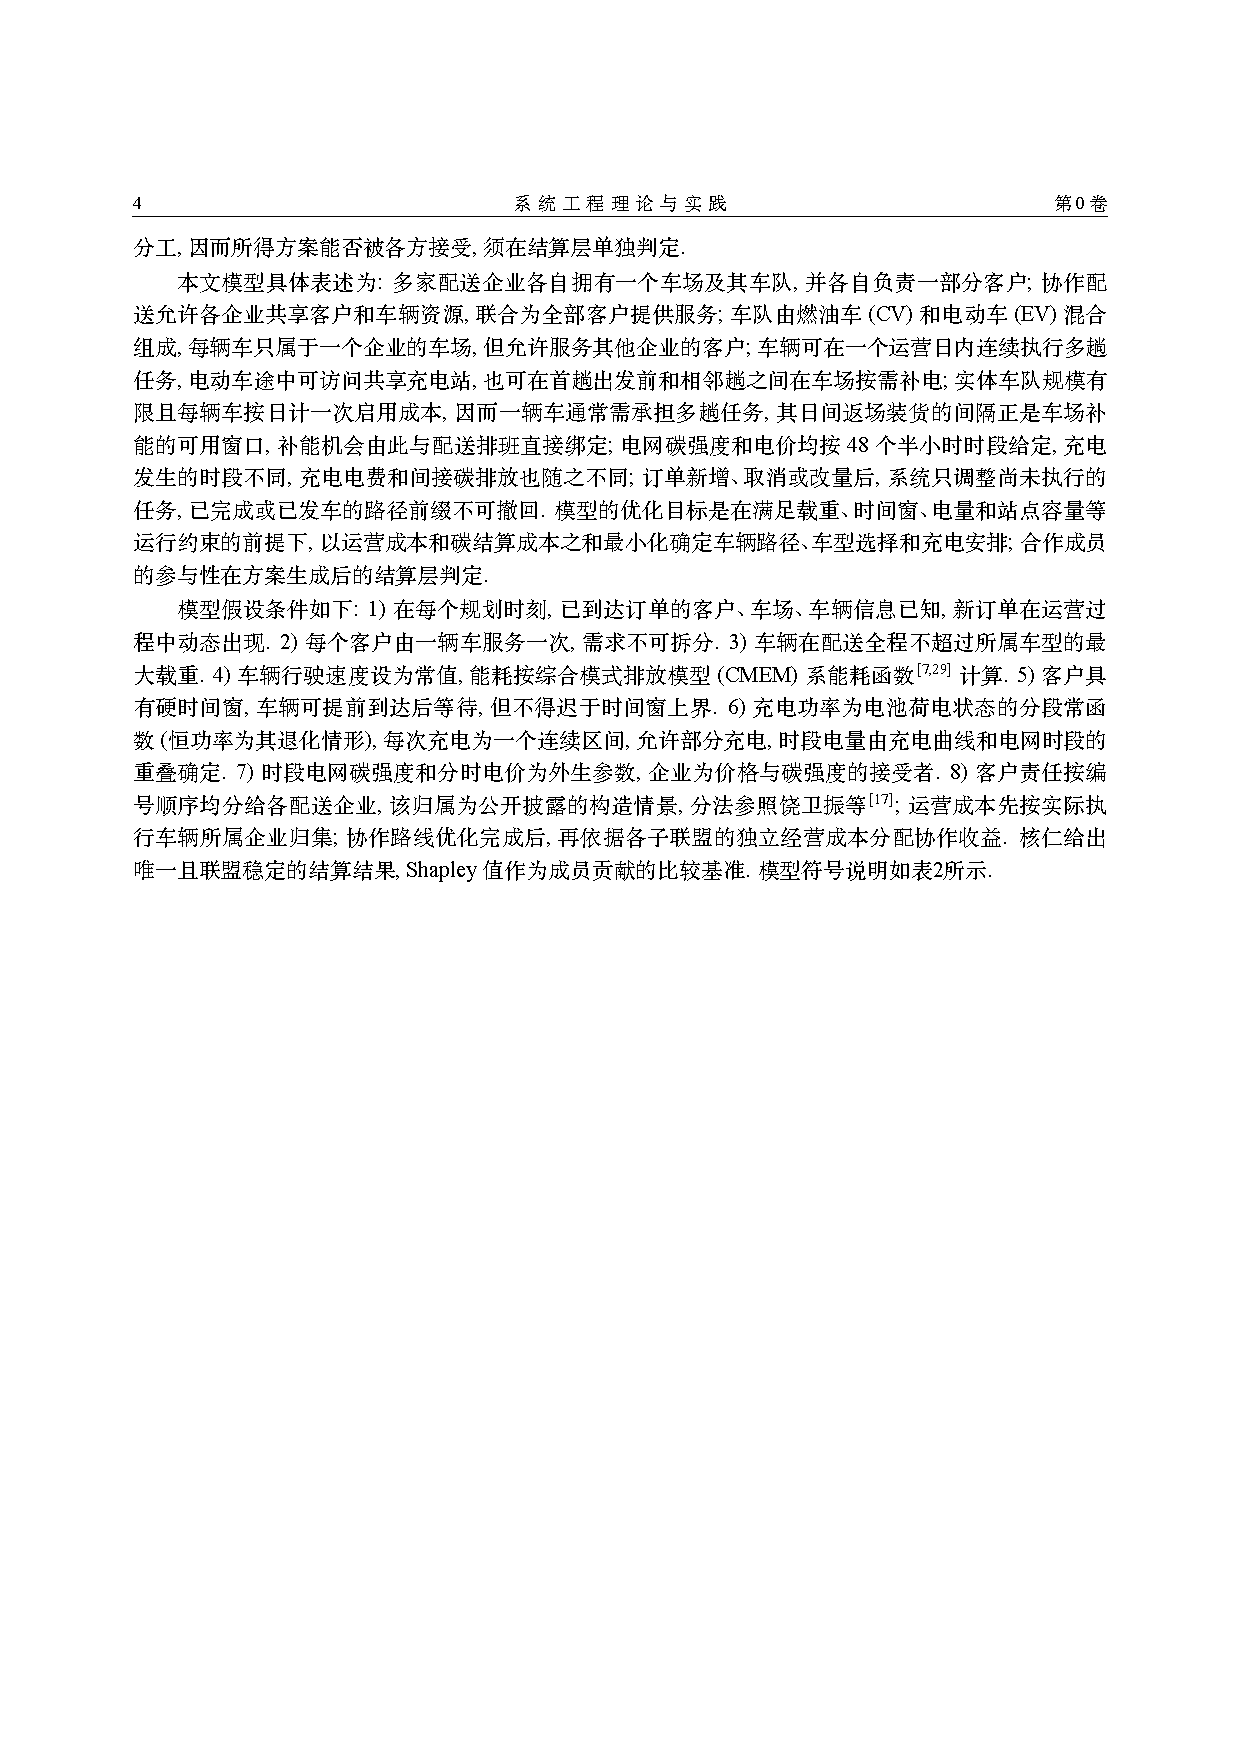
\includepdf[pages=-,scale=0.94,pagecommand={}]{source_excerpts/00_current_paper_model_pages_4_10.pdf}

\subsection{陈雨蝶等（2025）：同刊模型章表达}
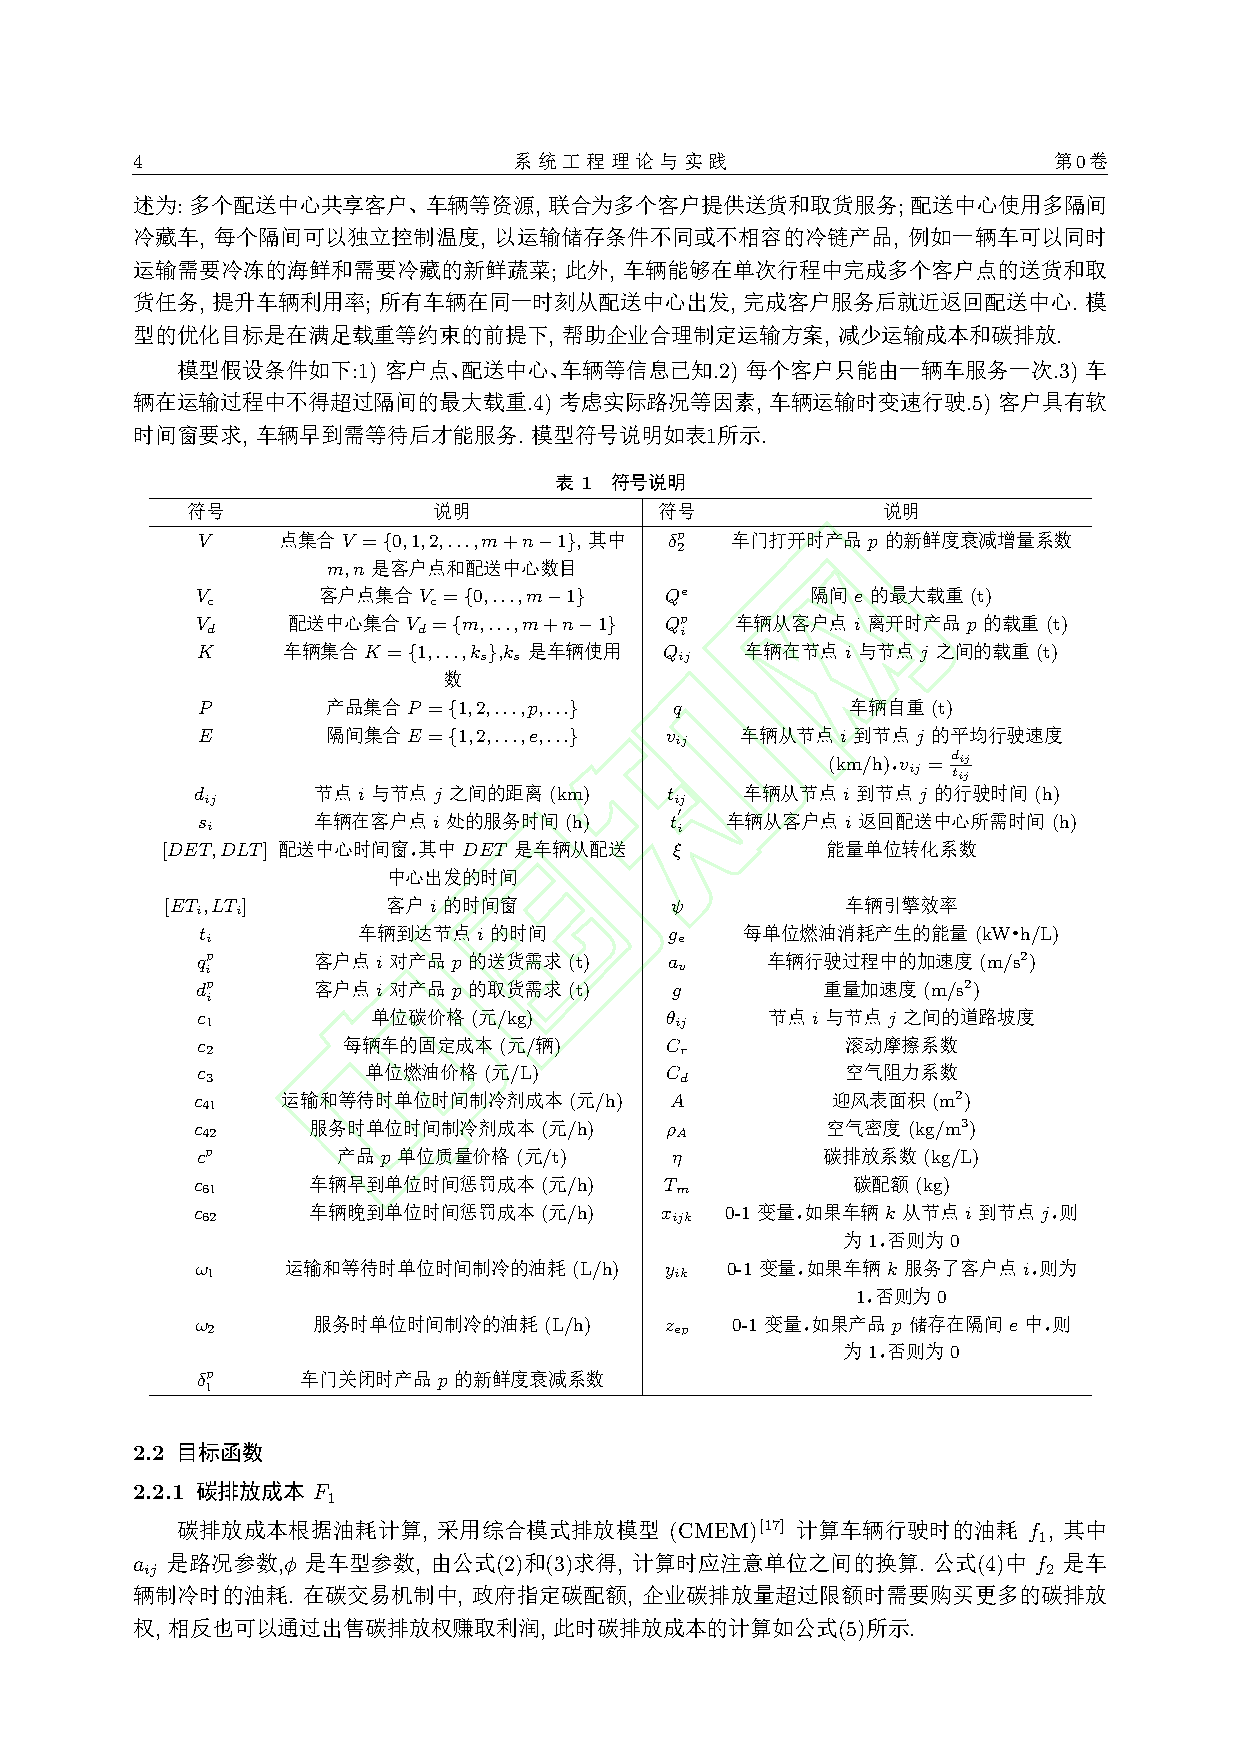
\includepdf[pages=-,scale=0.94,pagecommand={}]{source_excerpts/01_chen_yudie_2025_pages_5_8.pdf}

\subsection{陈婉茹等（2023）：混合车队、能耗与碳交易}
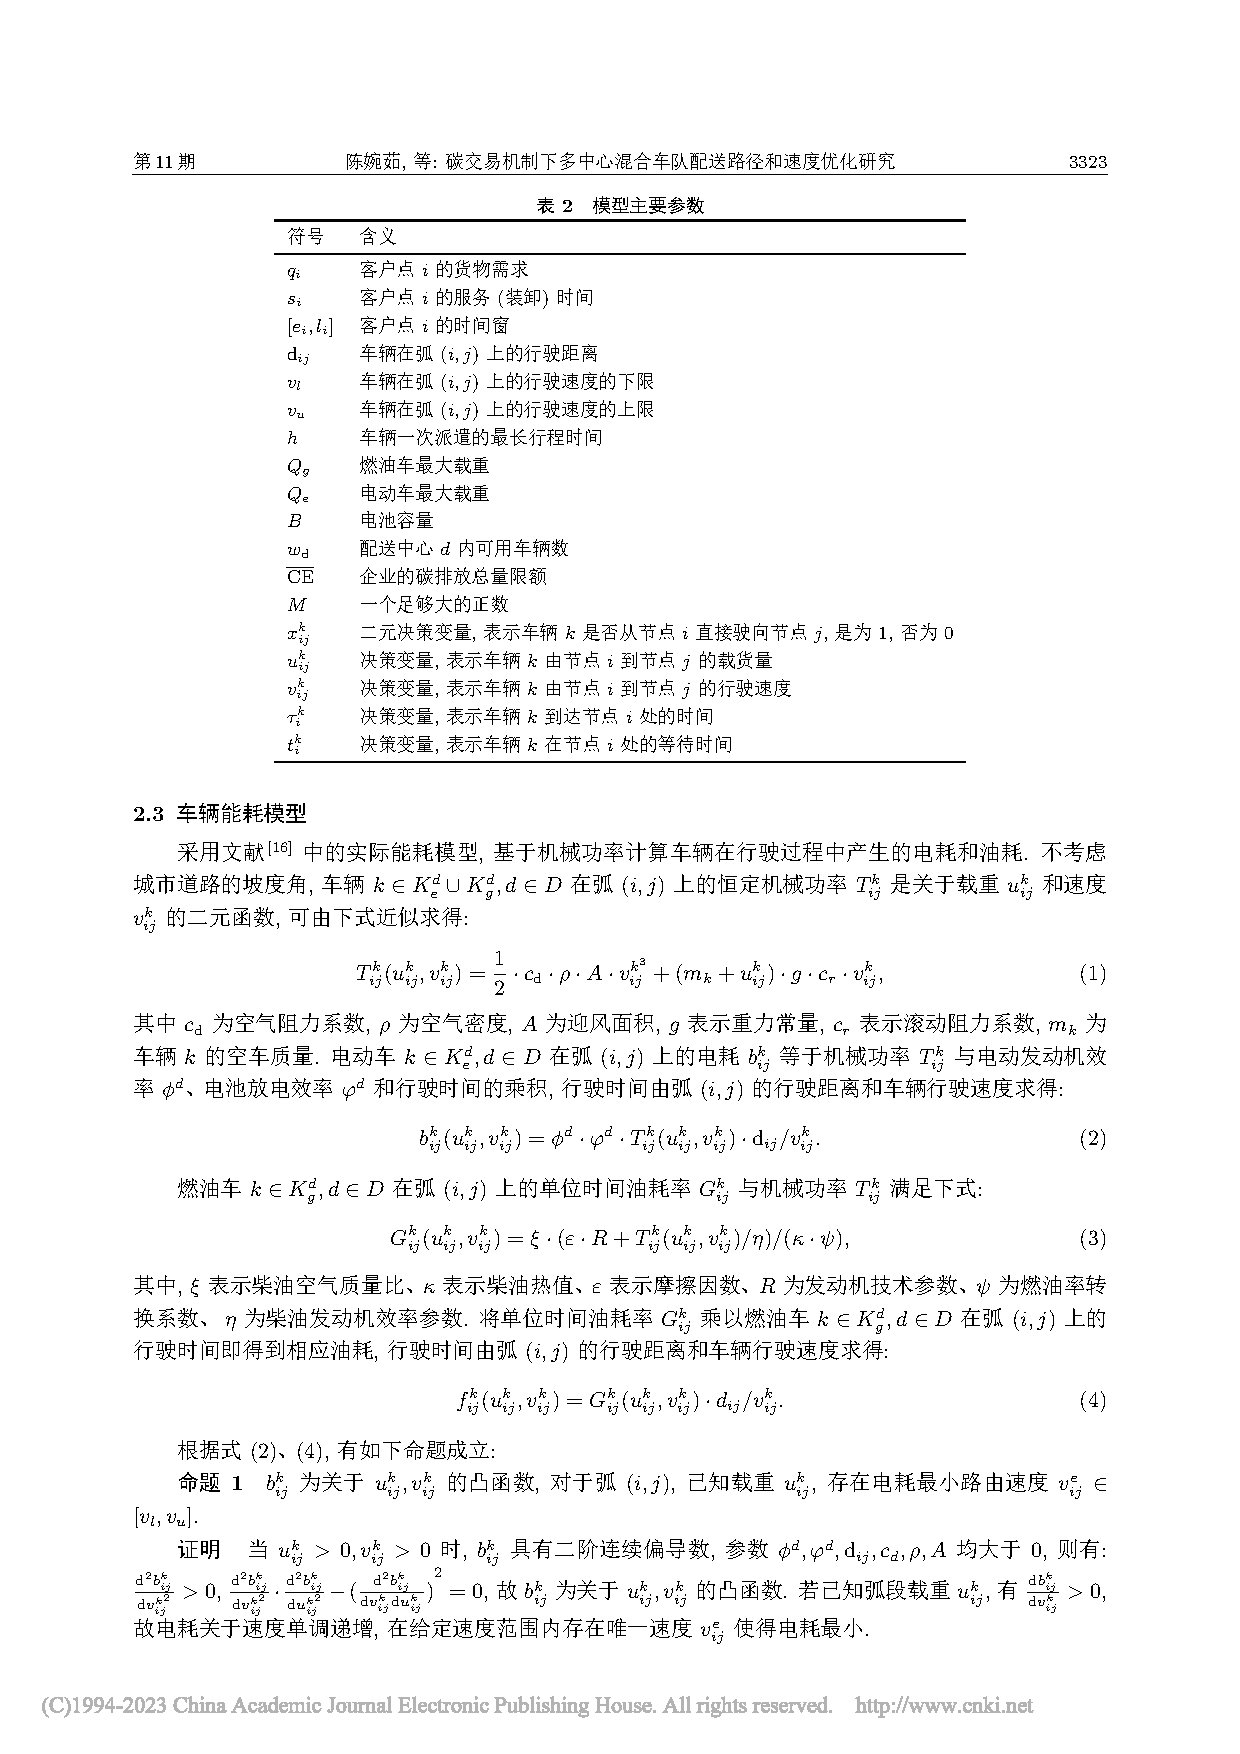
\includepdf[pages=-,scale=0.94,pagecommand={}]{source_excerpts/02_chen_wanru_2023_pages_4_6.pdf}

\subsection{Goeke--Schneider（2015）：混合车队能耗原式}
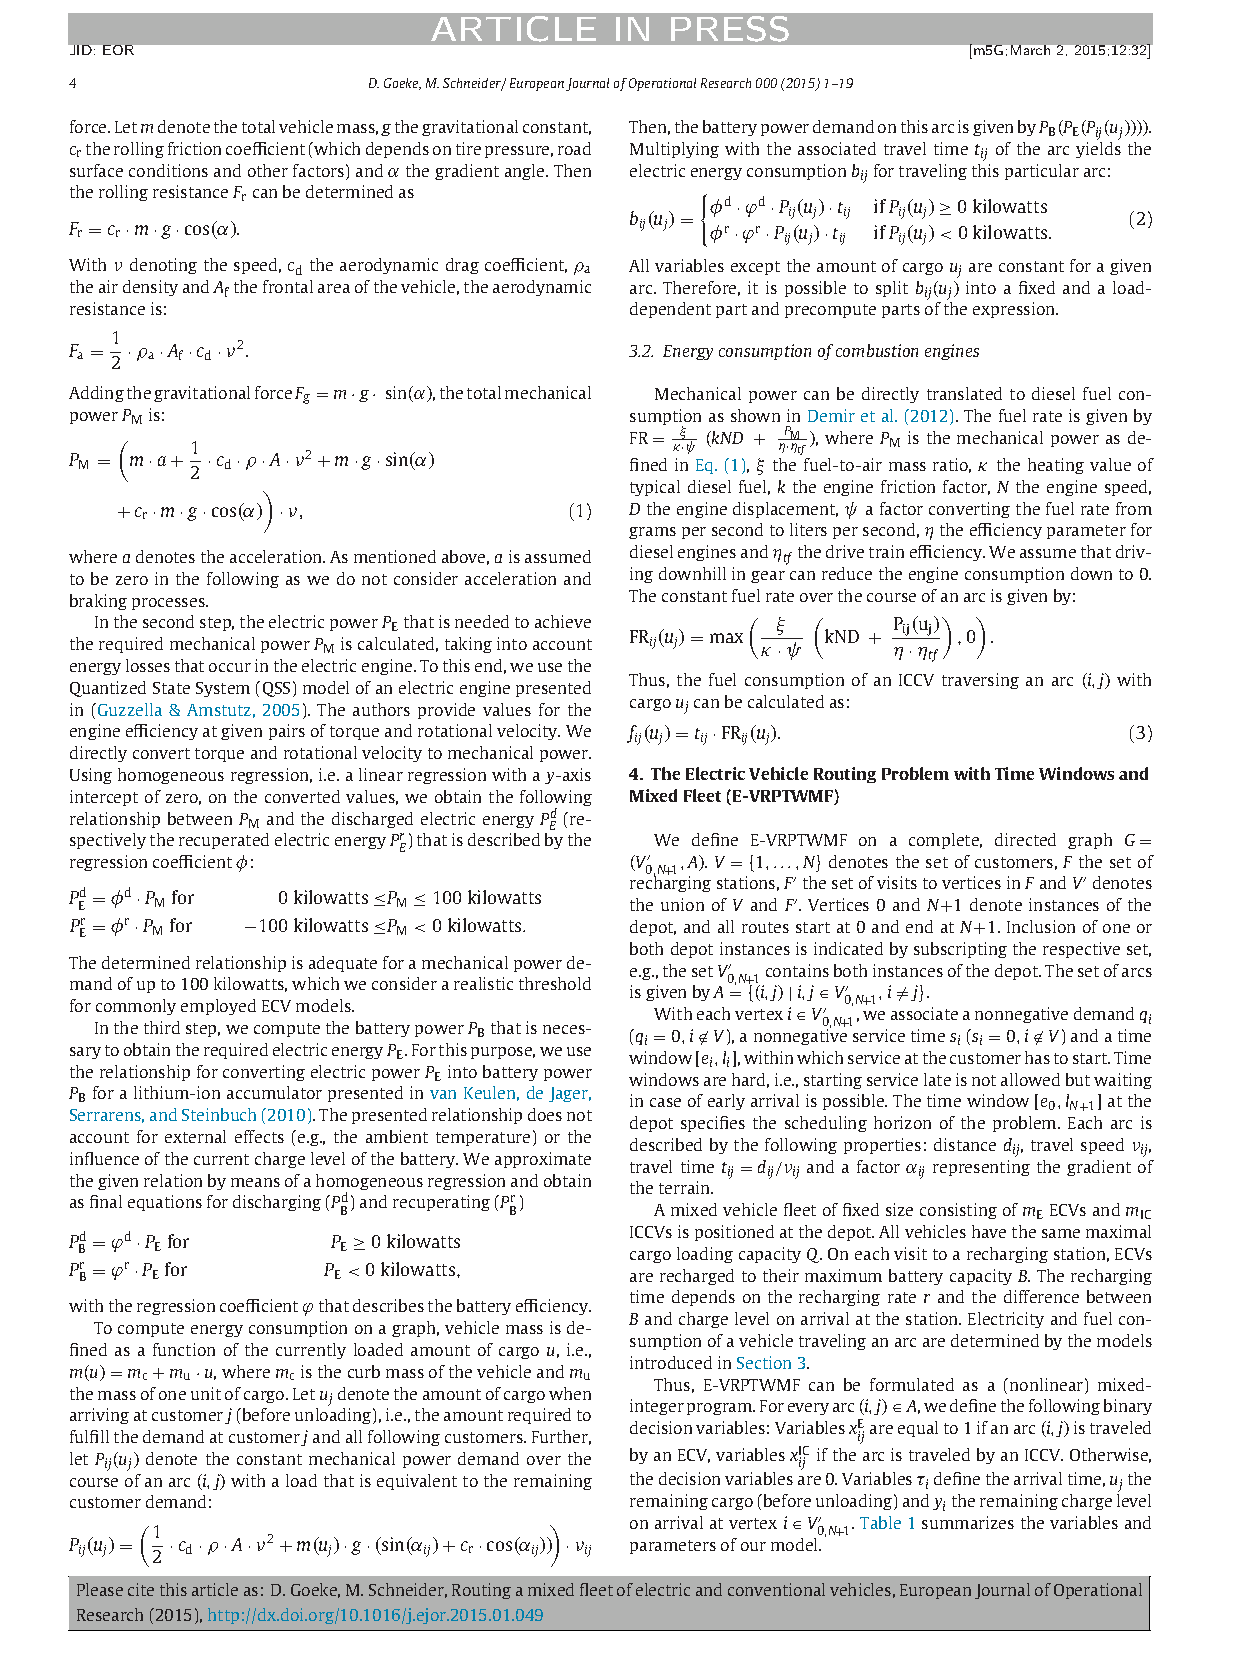
\includepdf[pages=-,scale=0.94,pagecommand={}]{source_excerpts/03_goeke_schneider_2015_pages_4_5.pdf}

\subsection{Zhen 等（2020）：多车场多趟原式}
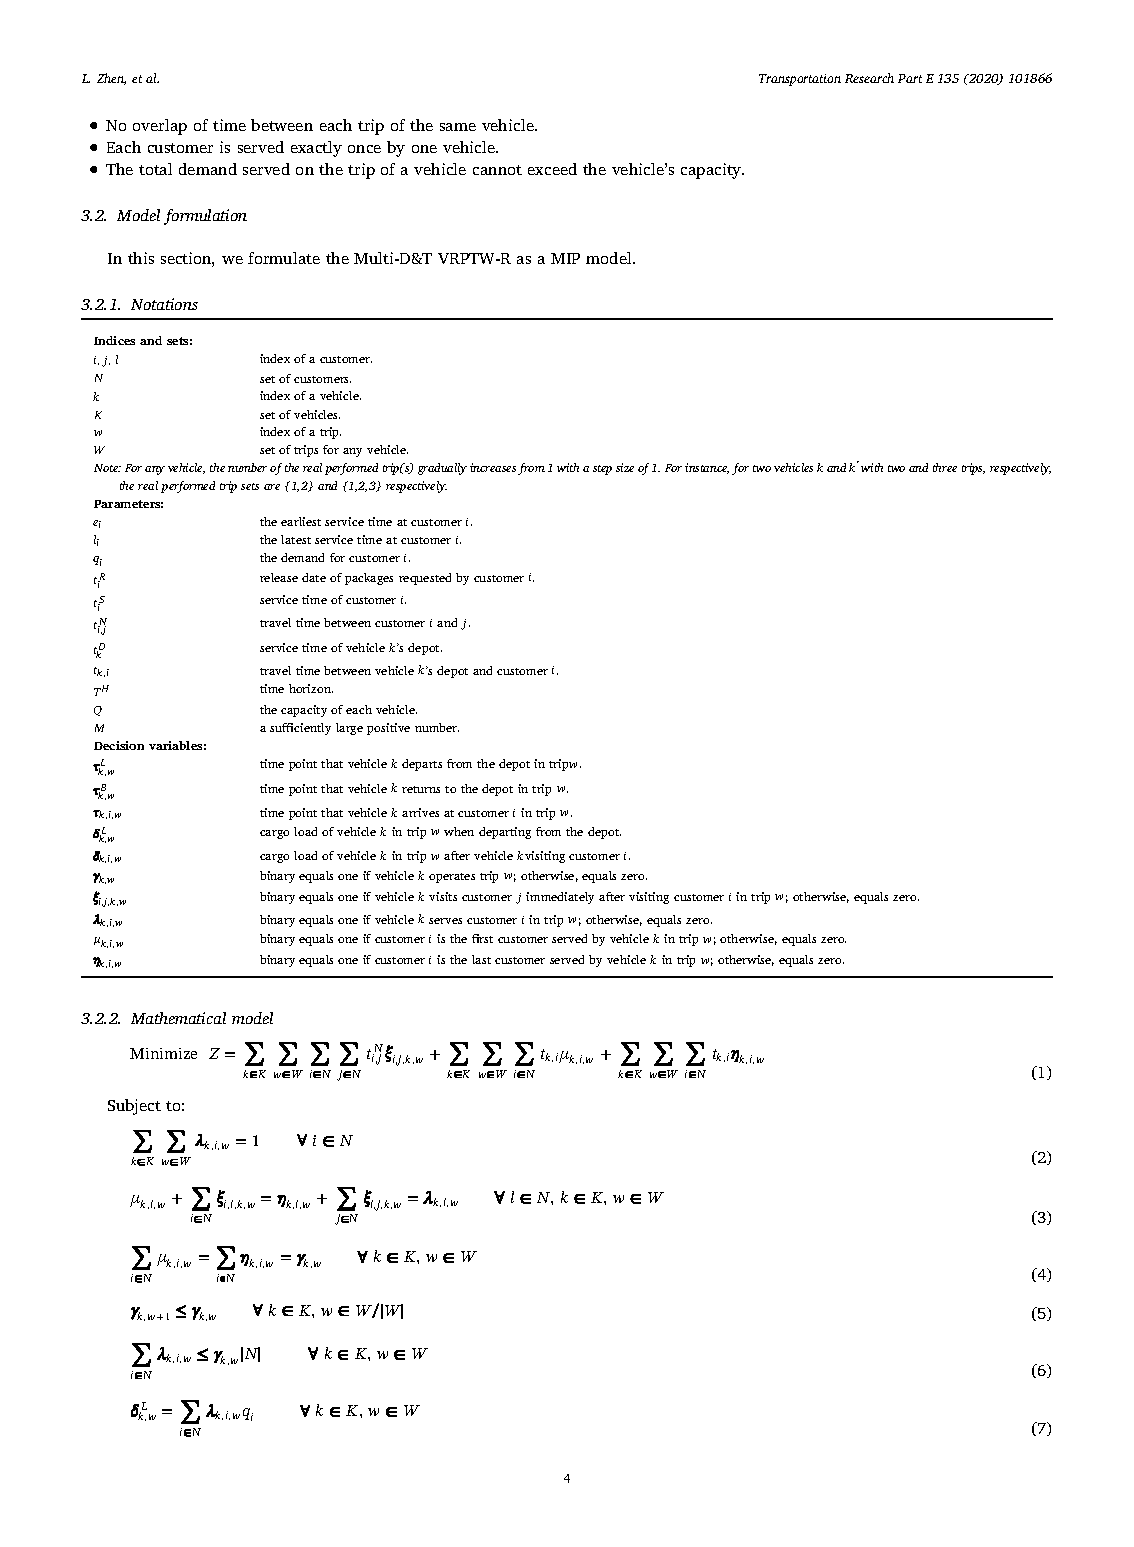
\includepdf[pages=-,scale=0.94,pagecommand={}]{source_excerpts/04_zhen_2020_pages_4_5.pdf}

\subsection{Keskin--Çatay（2016）：线性部分充电原式}
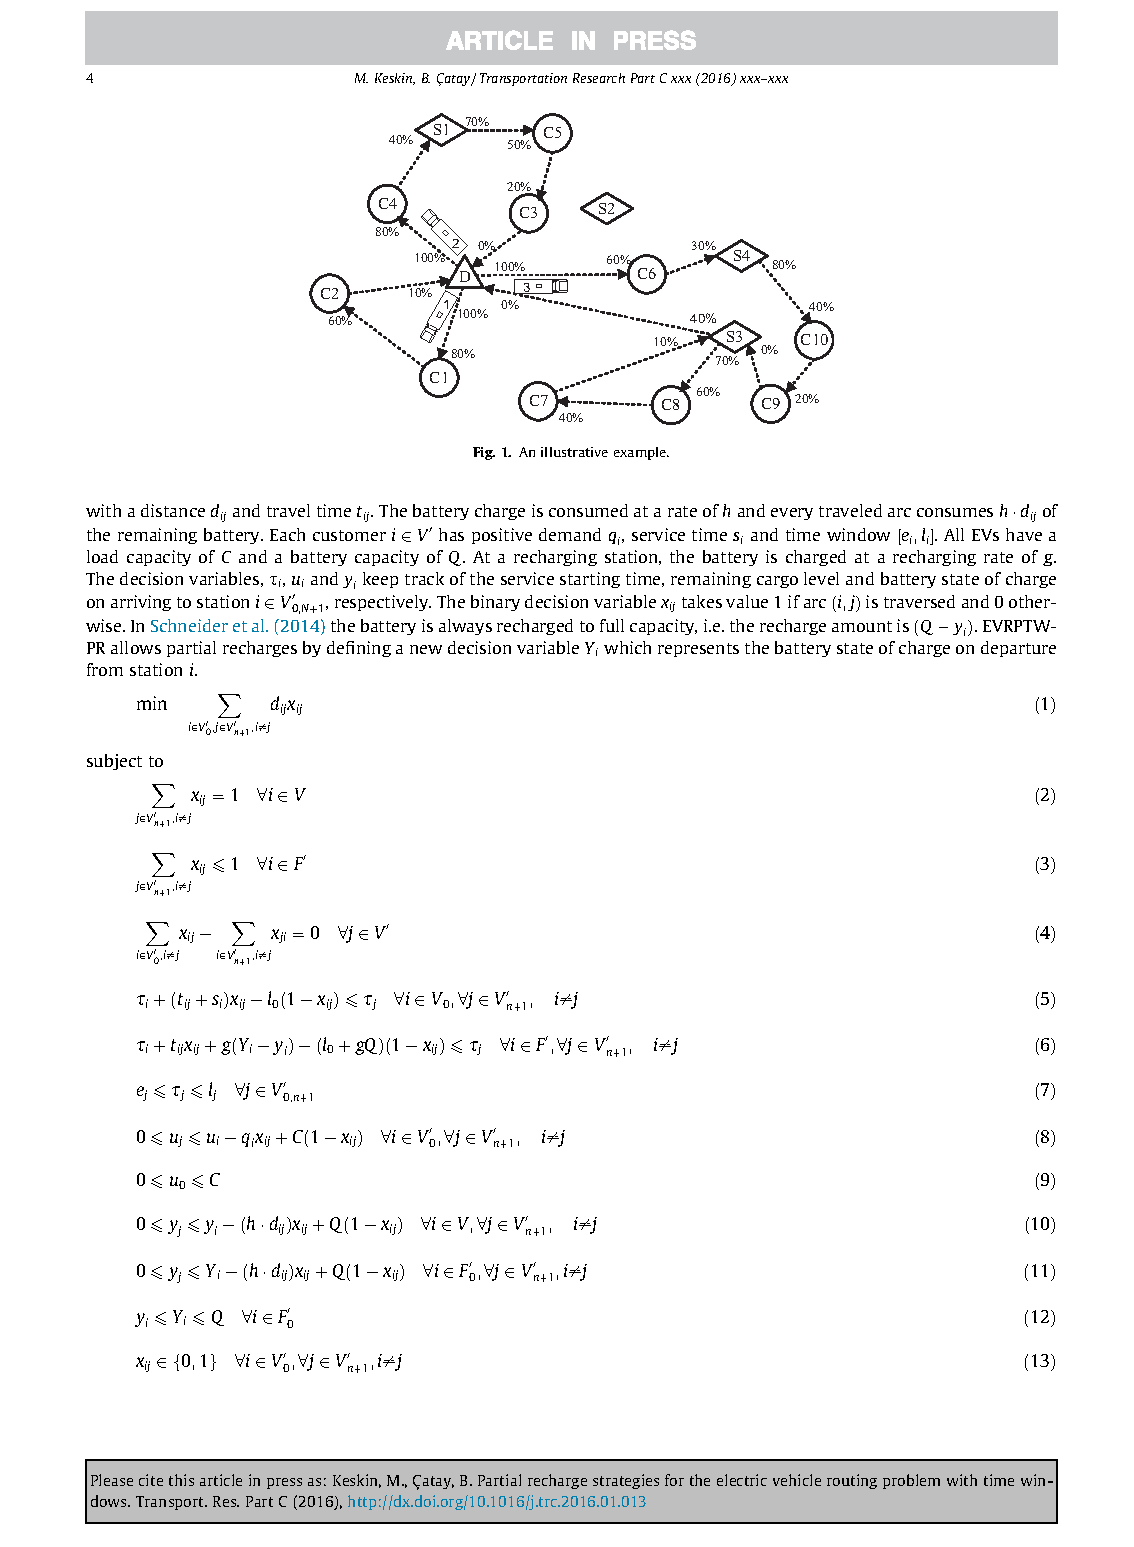
\includepdf[pages=-,scale=0.94,pagecommand={}]{source_excerpts/05_keskin_catay_2016_pages_4_5.pdf}

\subsection{Montoya 等（2017）：非线性充电路径模型}
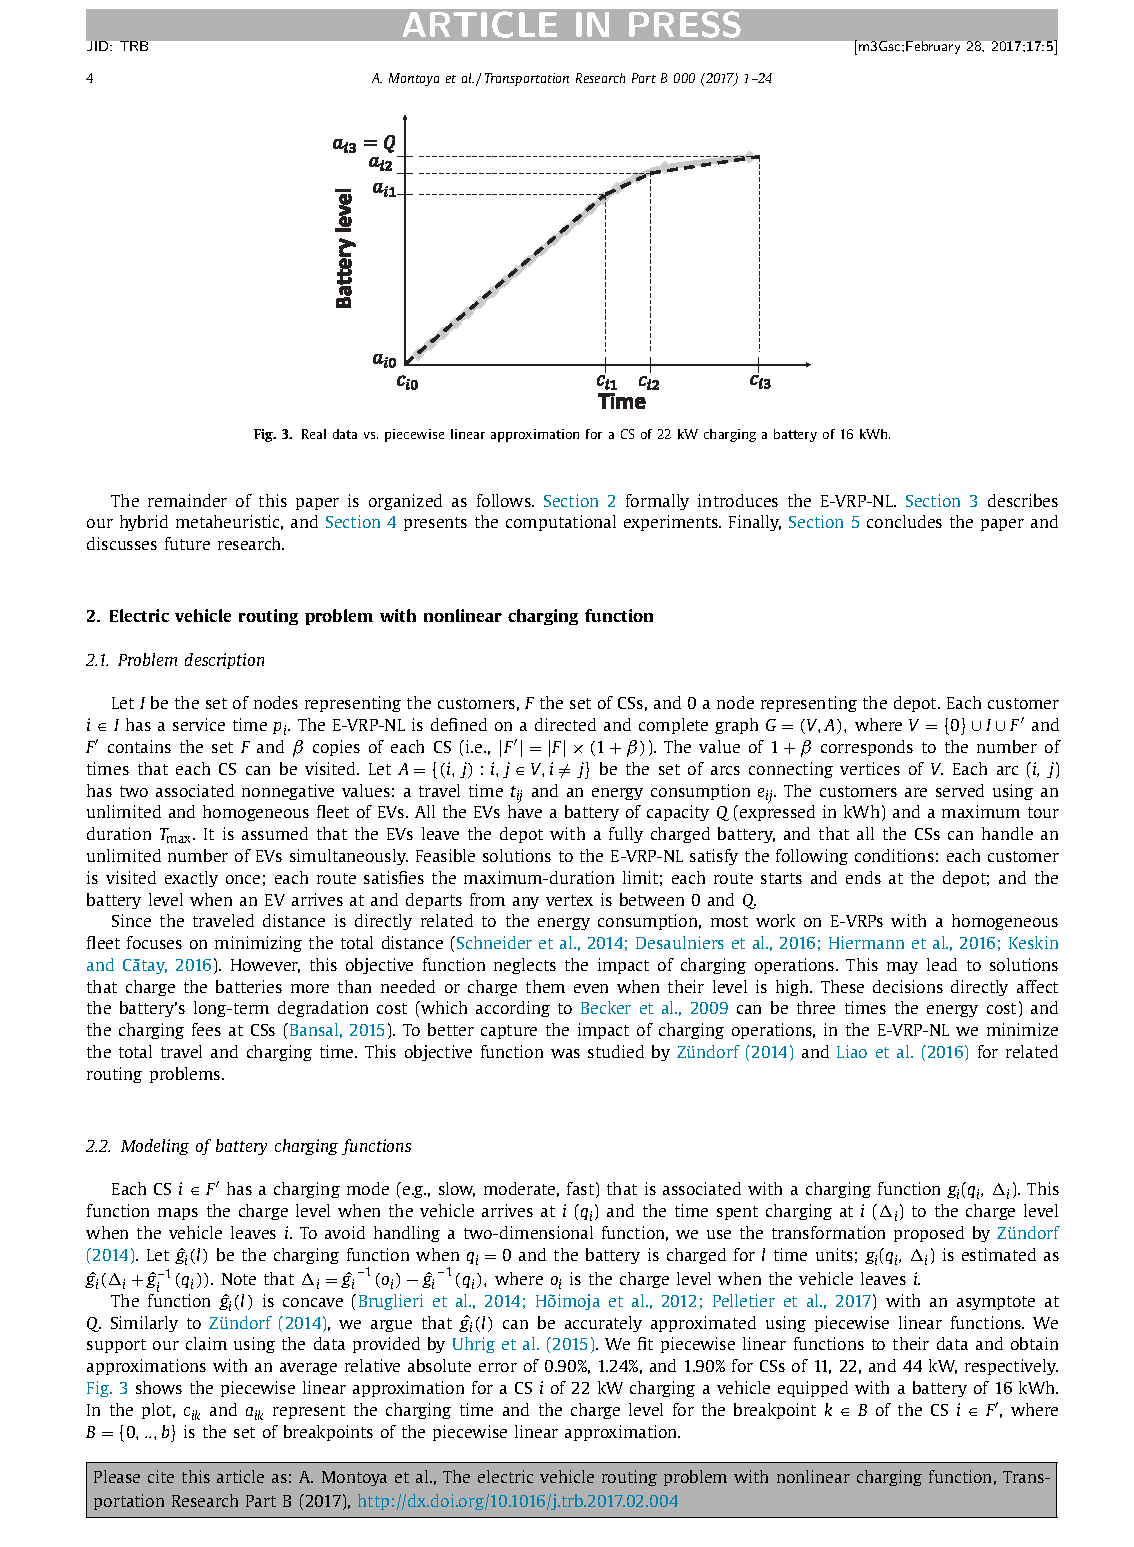
\includepdf[pages=-,scale=0.94,pagecommand={}]{source_excerpts/06_montoya_2017_pages_4_7.pdf}

\subsection{Diefenbach 等（2023）：非线性充电排班模型}
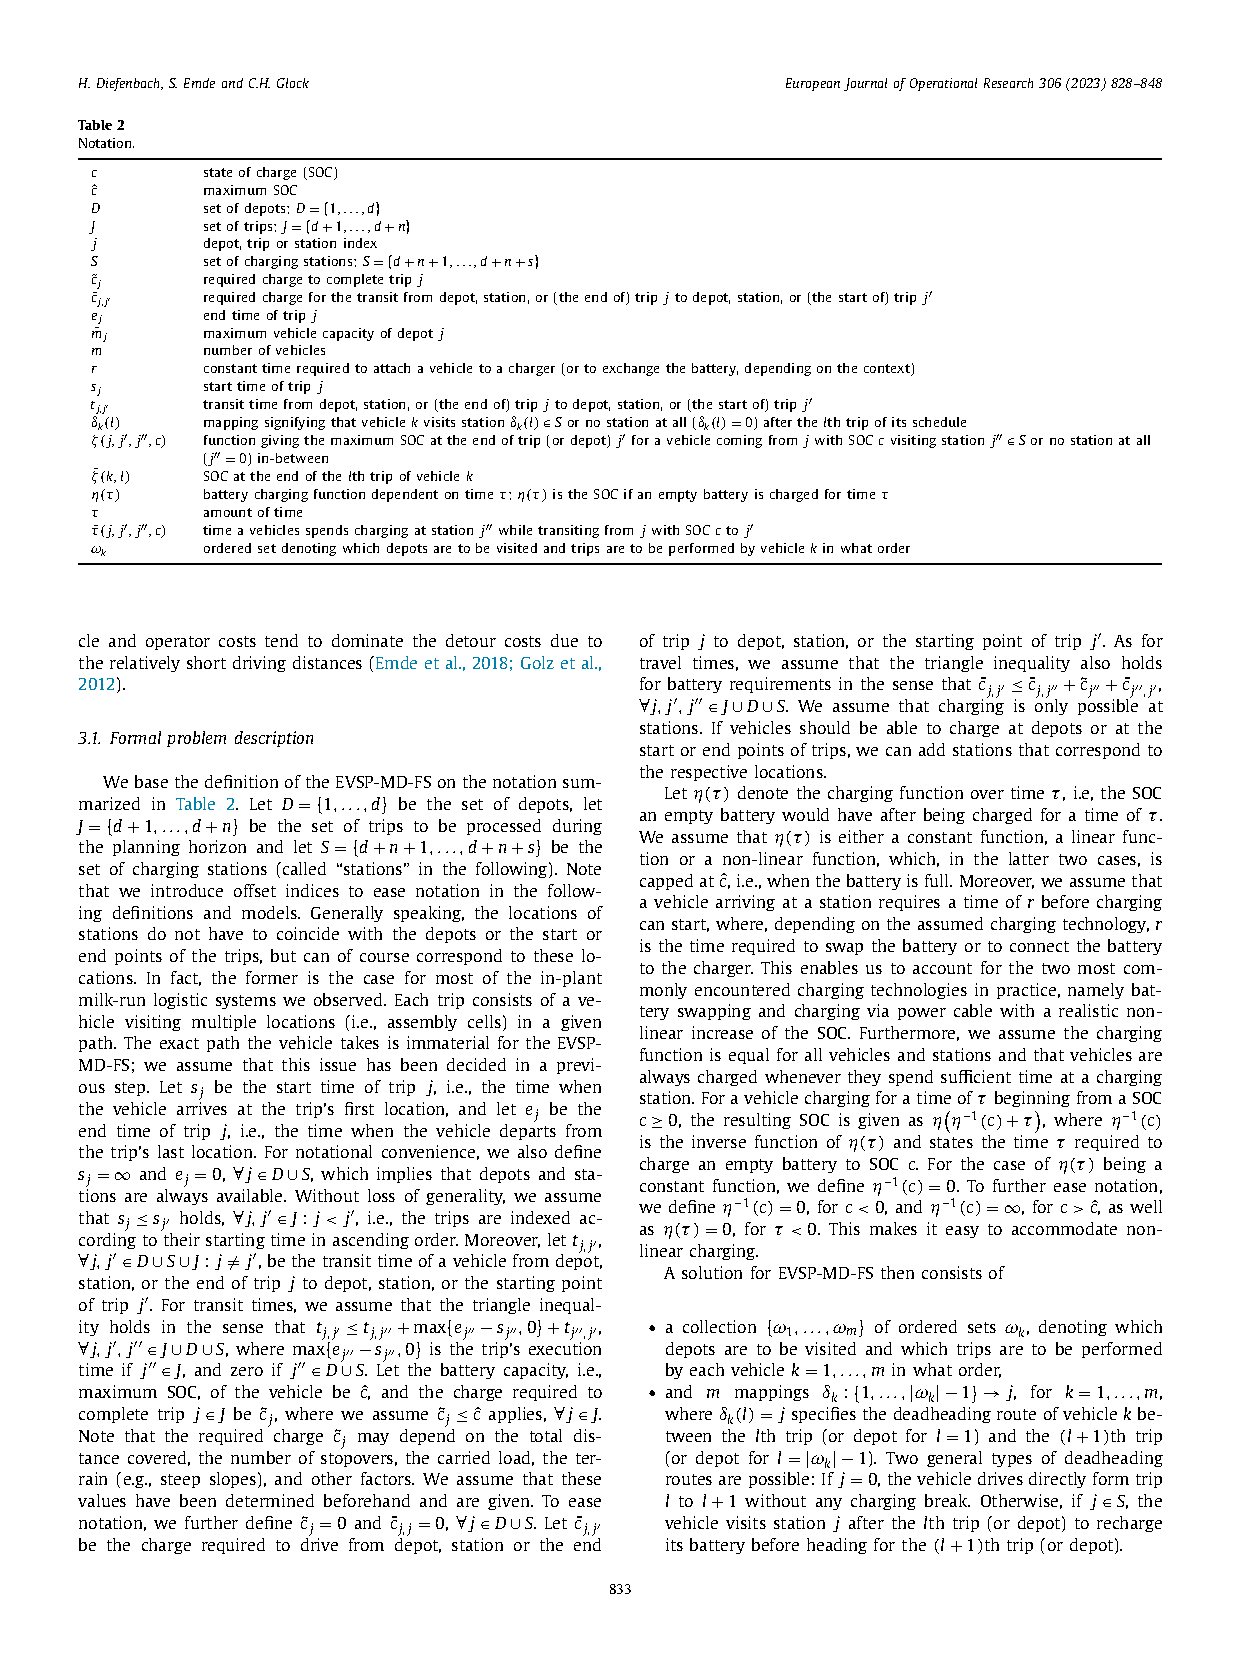
\includepdf[pages=-,scale=0.94,pagecommand={}]{source_excerpts/07_diefenbach_2023_pages_6_9.pdf}

\subsection{Froger 等（2022）：容量受限充电站模型}
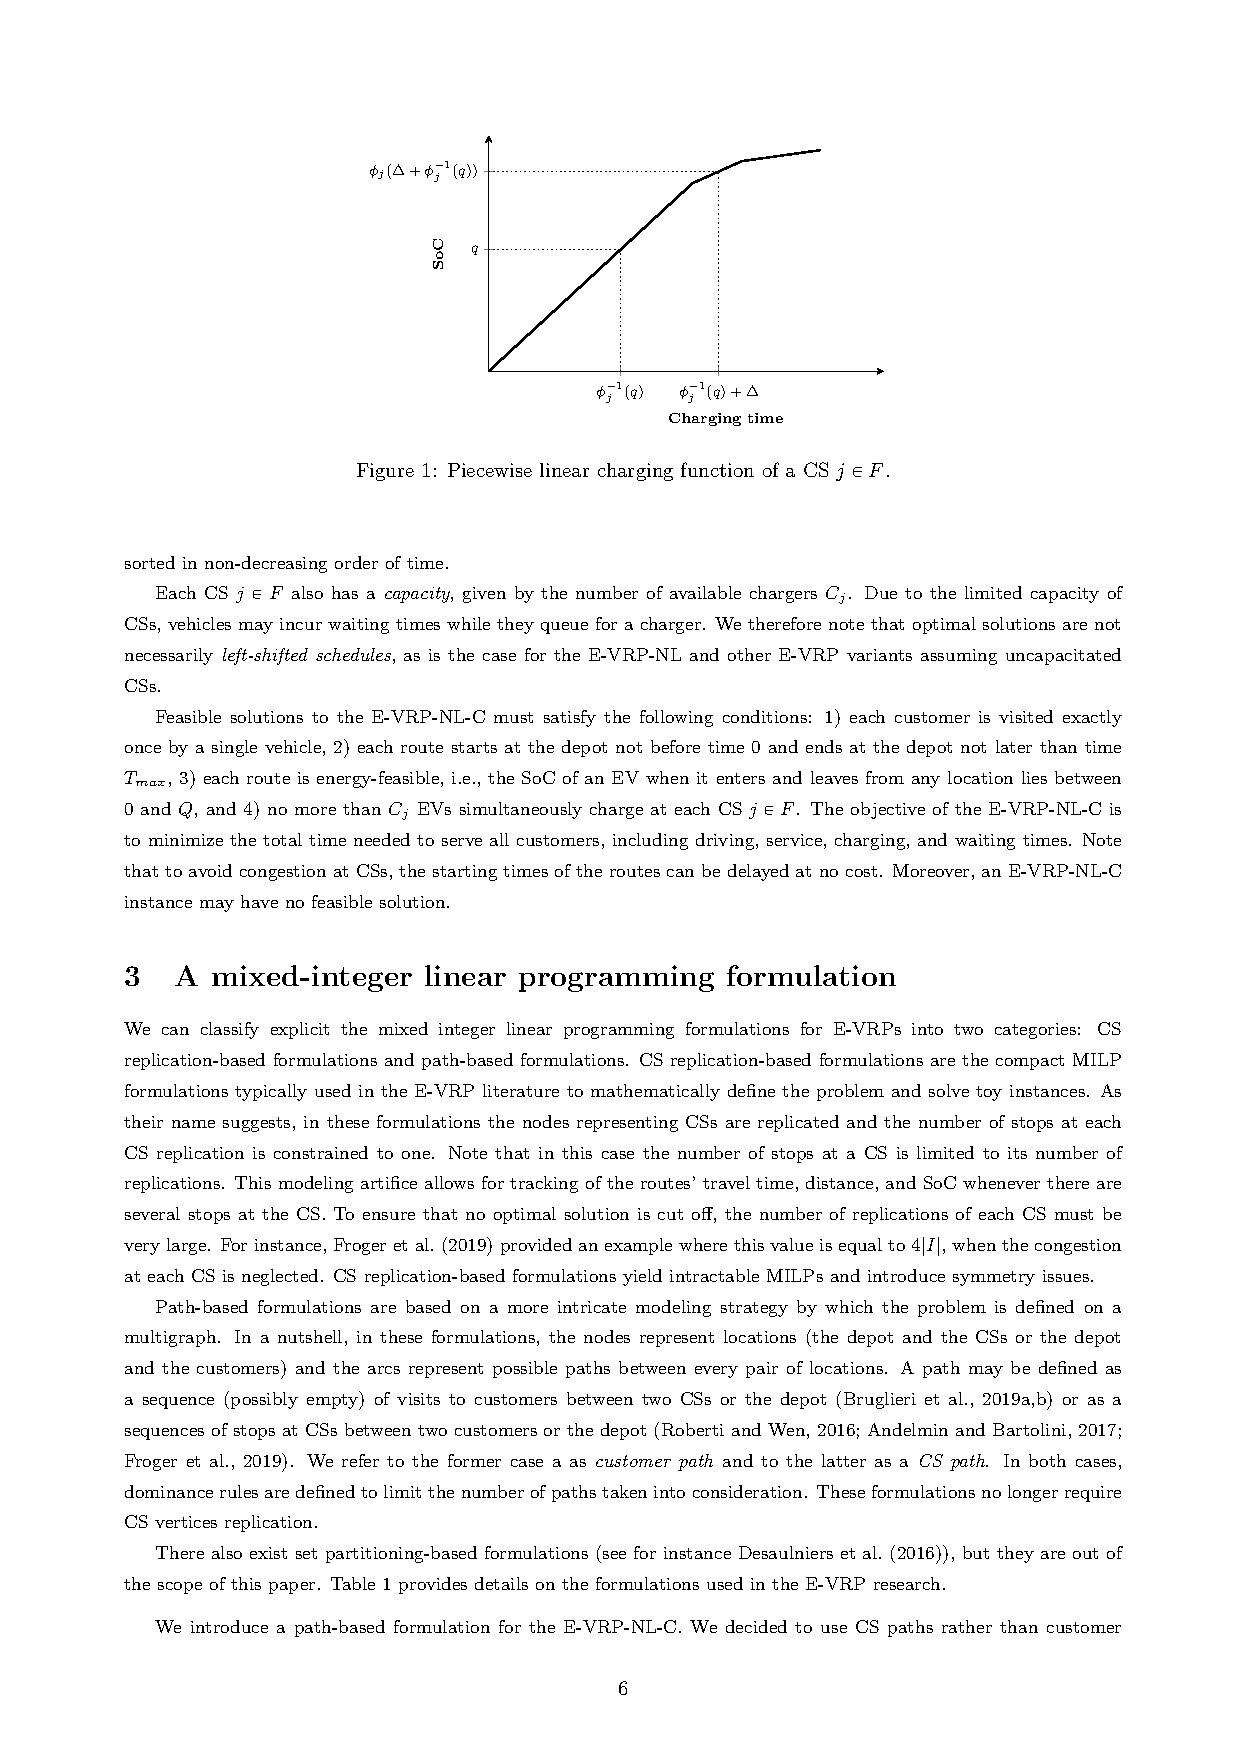
\includepdf[pages=-,scale=0.94,pagecommand={}]{source_excerpts/08_froger_2022_pages_7_10.pdf}

\subsection{邱莹莹（2024）：混合车队与动态需求模型}
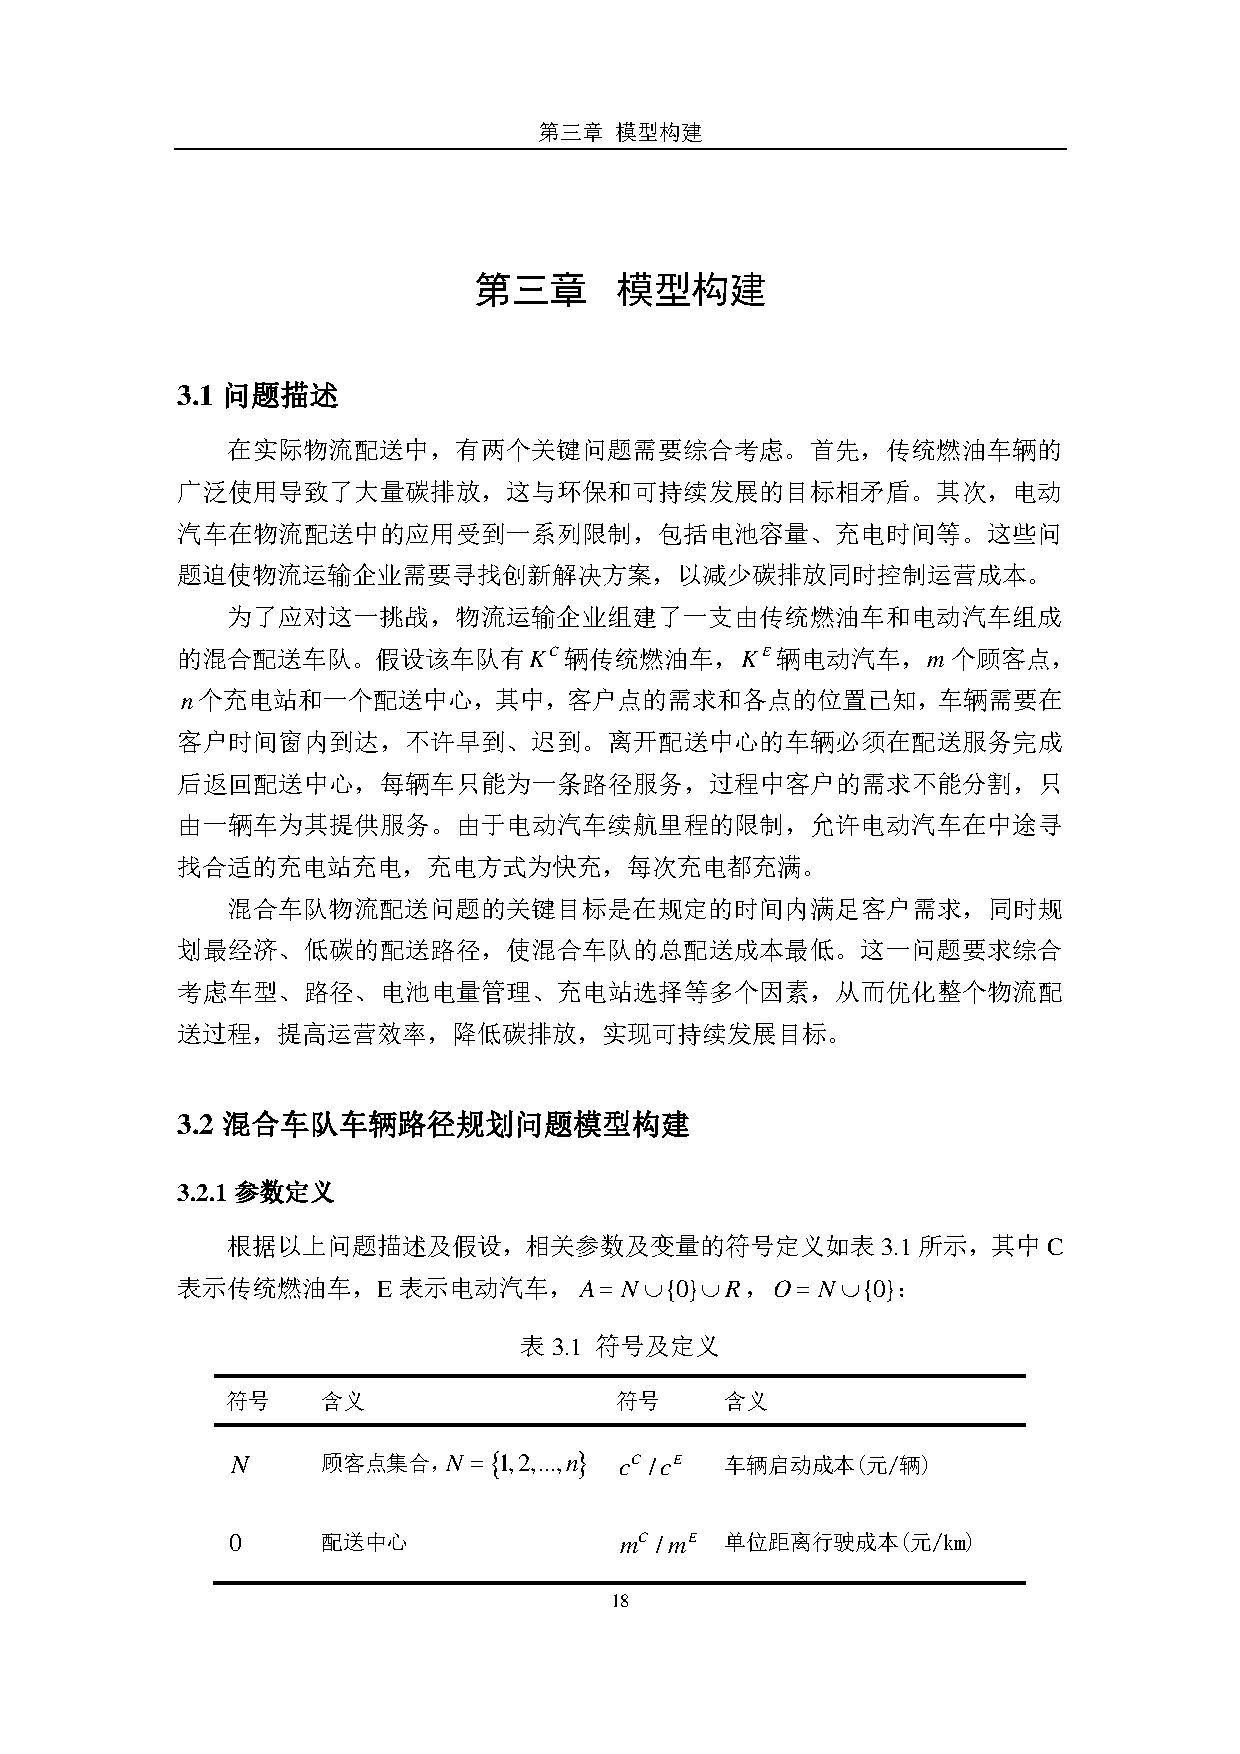
\includepdf[pages=-,scale=0.94,pagecommand={}]{source_excerpts/09_qiu_2024_pages_30_39.pdf}

\subsection{饶卫振等（2022）：协同配送与成本分摊模型}
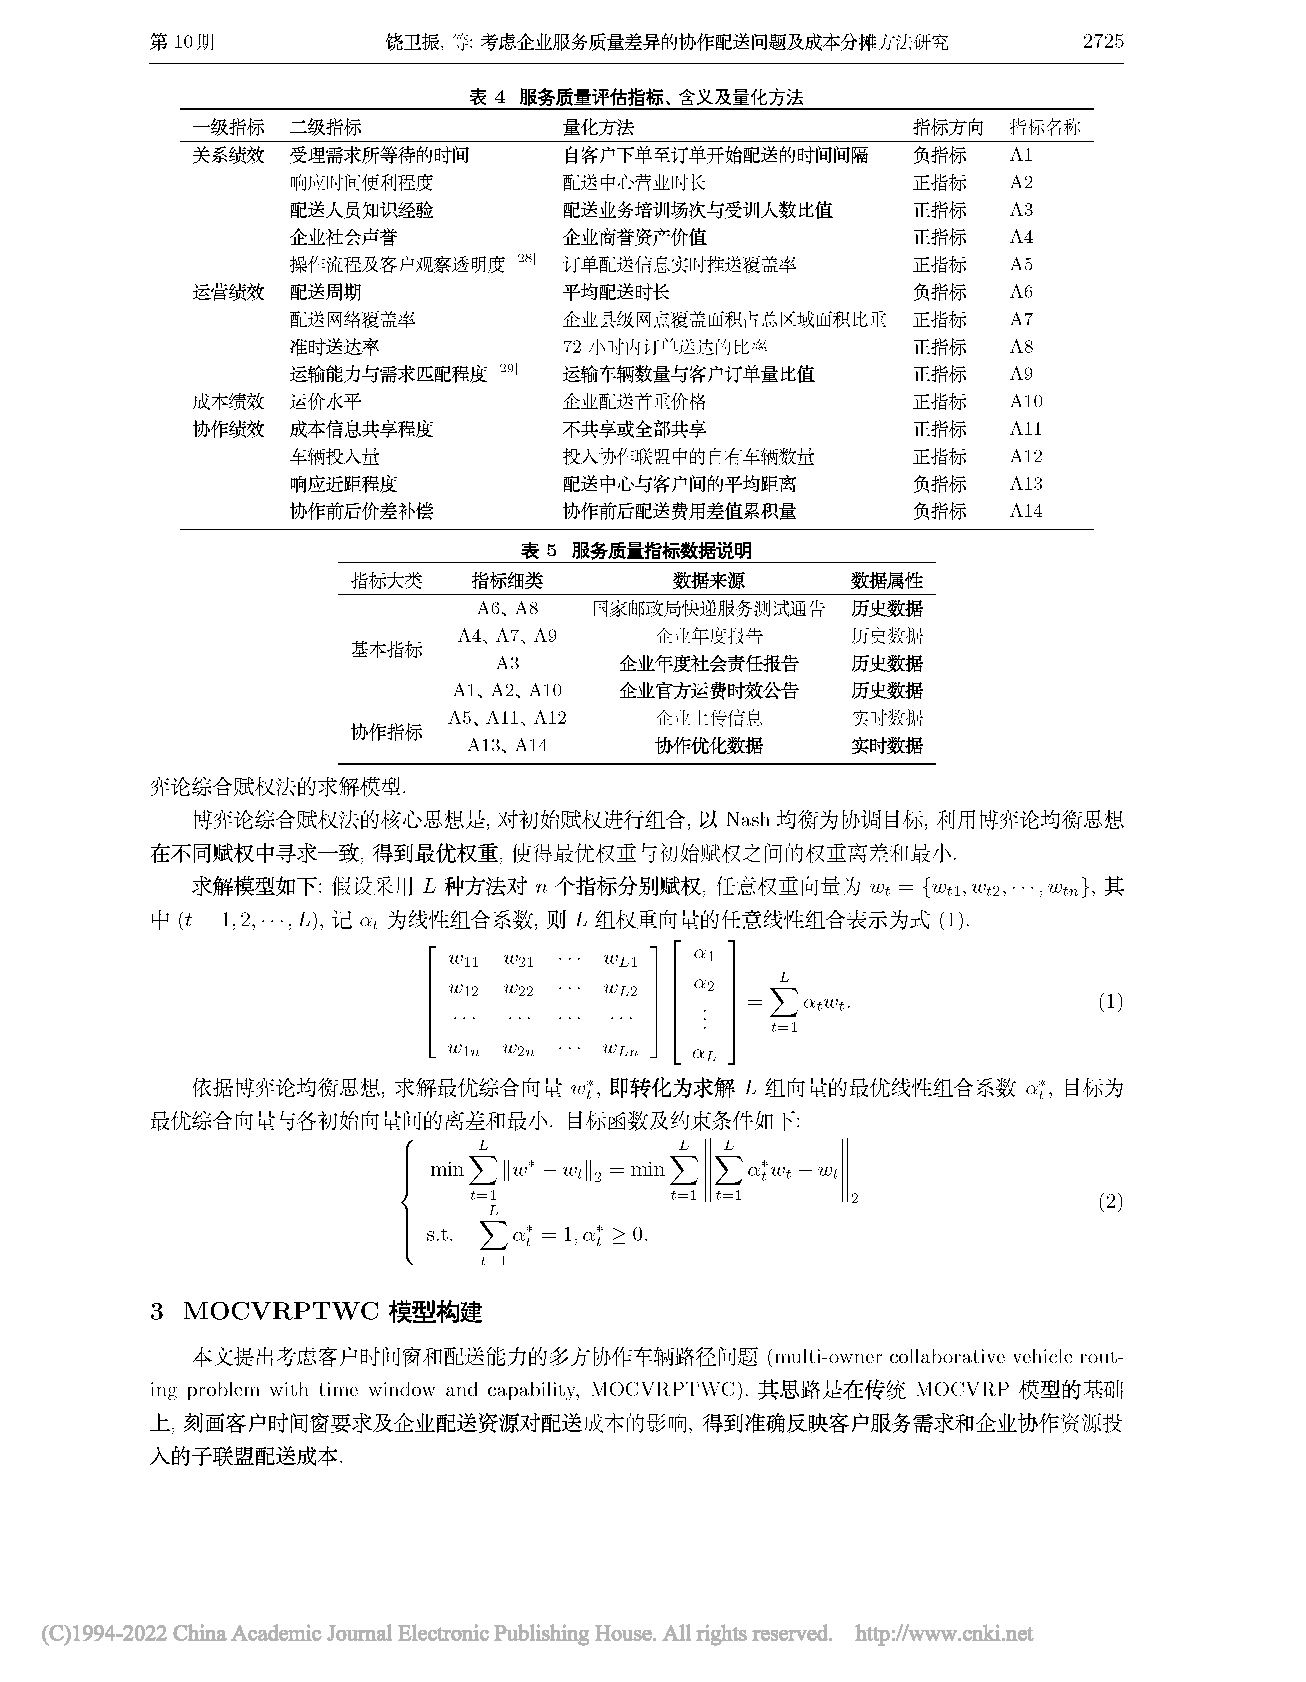
\includepdf[pages=-,scale=0.94,pagecommand={}]{source_excerpts/10_rao_2022_pages_5_9.pdf}

\subsection{胡路等（2025）：充电桩排队与路径模型}
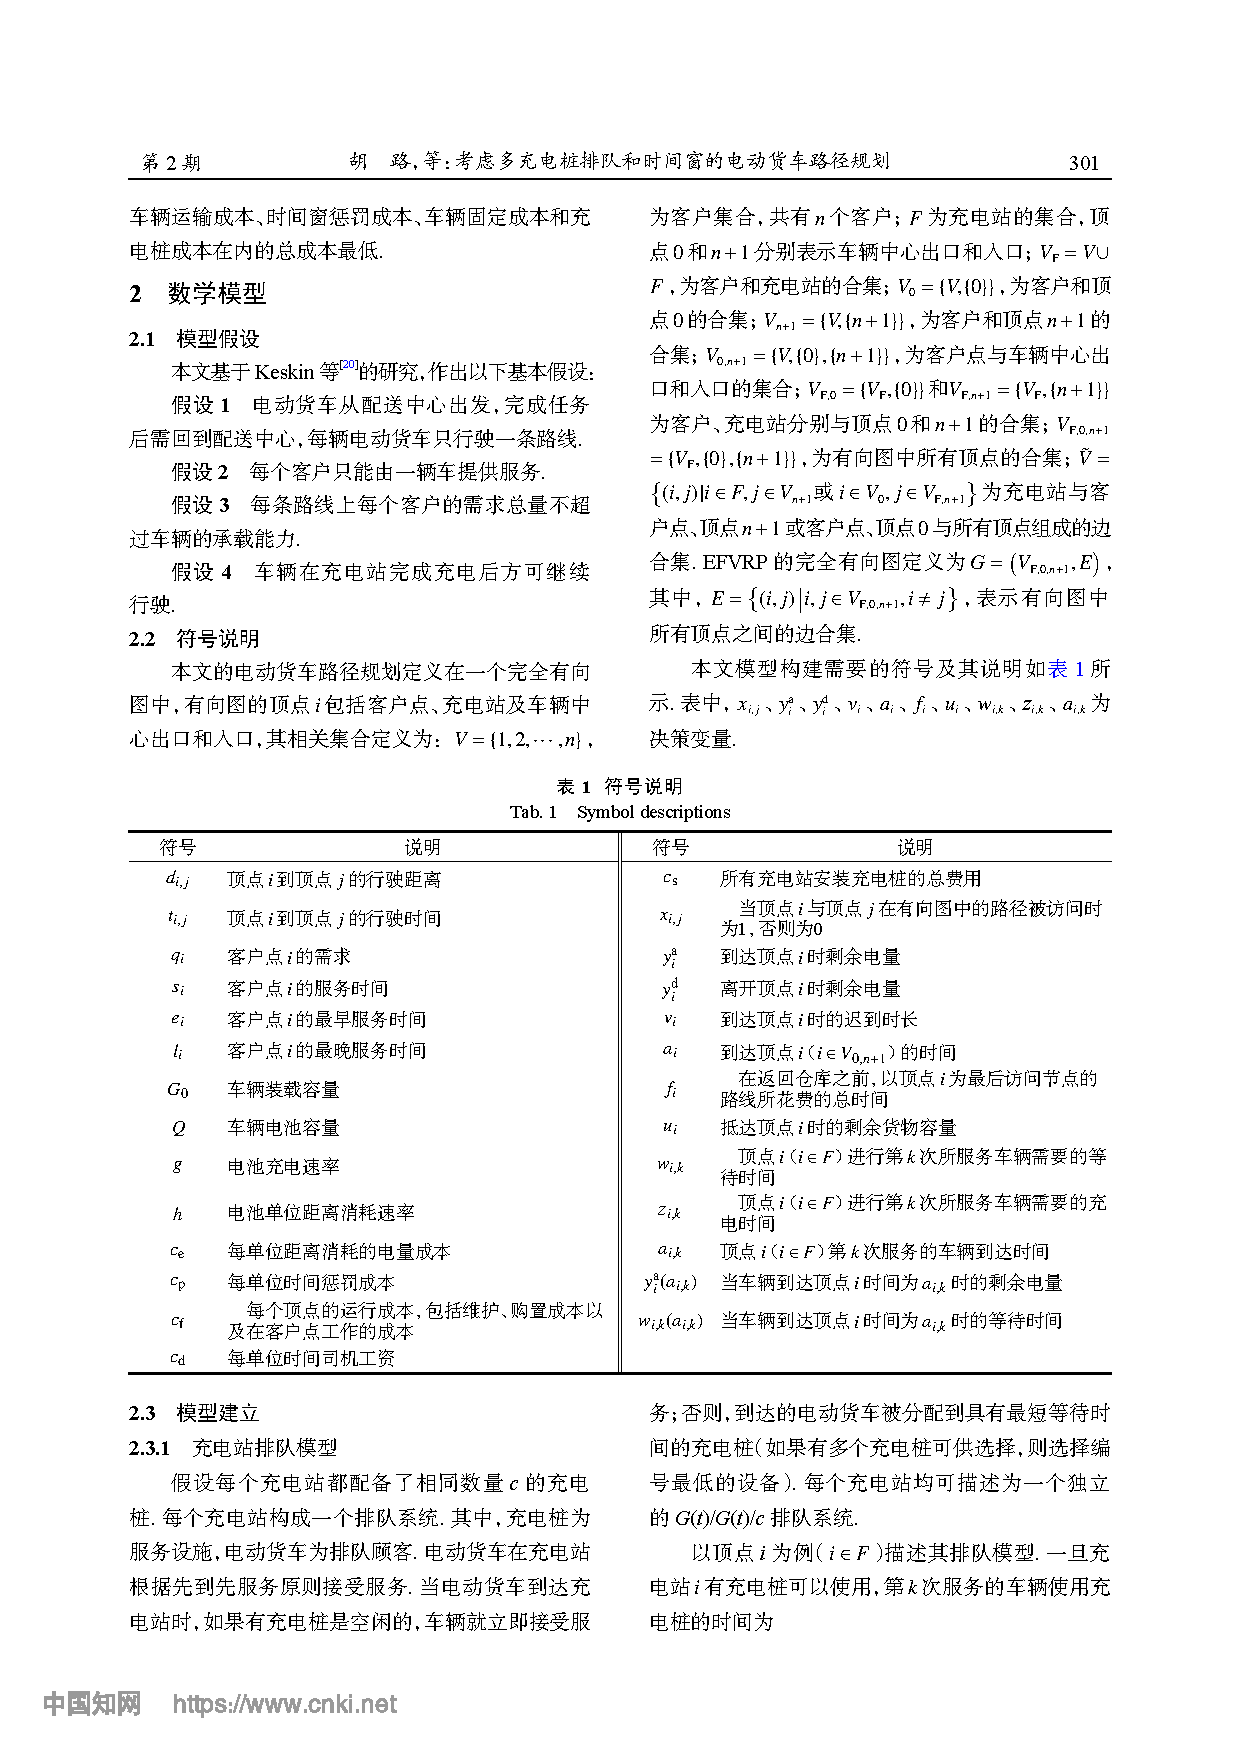
\includepdf[pages=-,scale=0.94,pagecommand={}]{source_excerpts/11_hu_2025_pages_3_4.pdf}

\subsection{Cheng 等（2022）：分时碳强度充电模型}
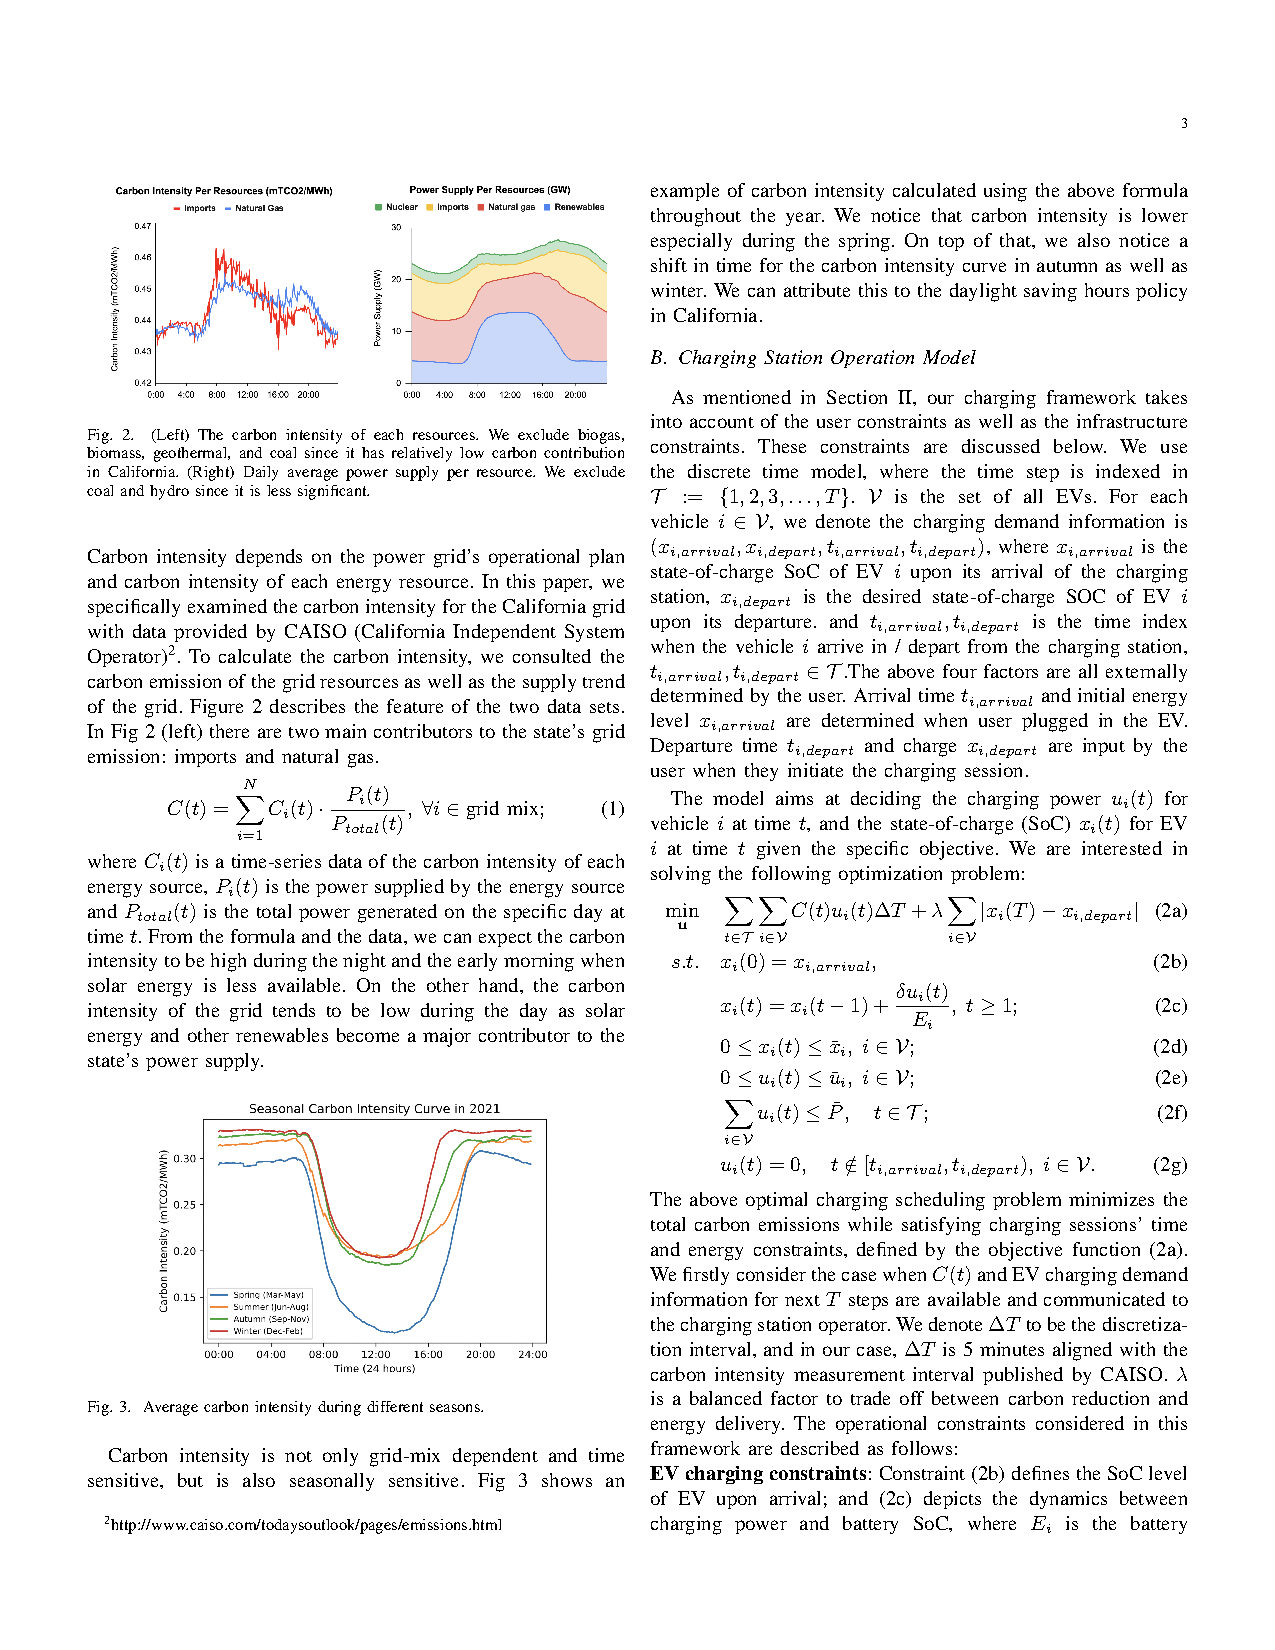
\includepdf[pages=-,scale=0.94,pagecommand={}]{source_excerpts/12_cheng_2022_pages_3_4.pdf}

\subsection{Lin 等（2021）：分时电价充放电模型}
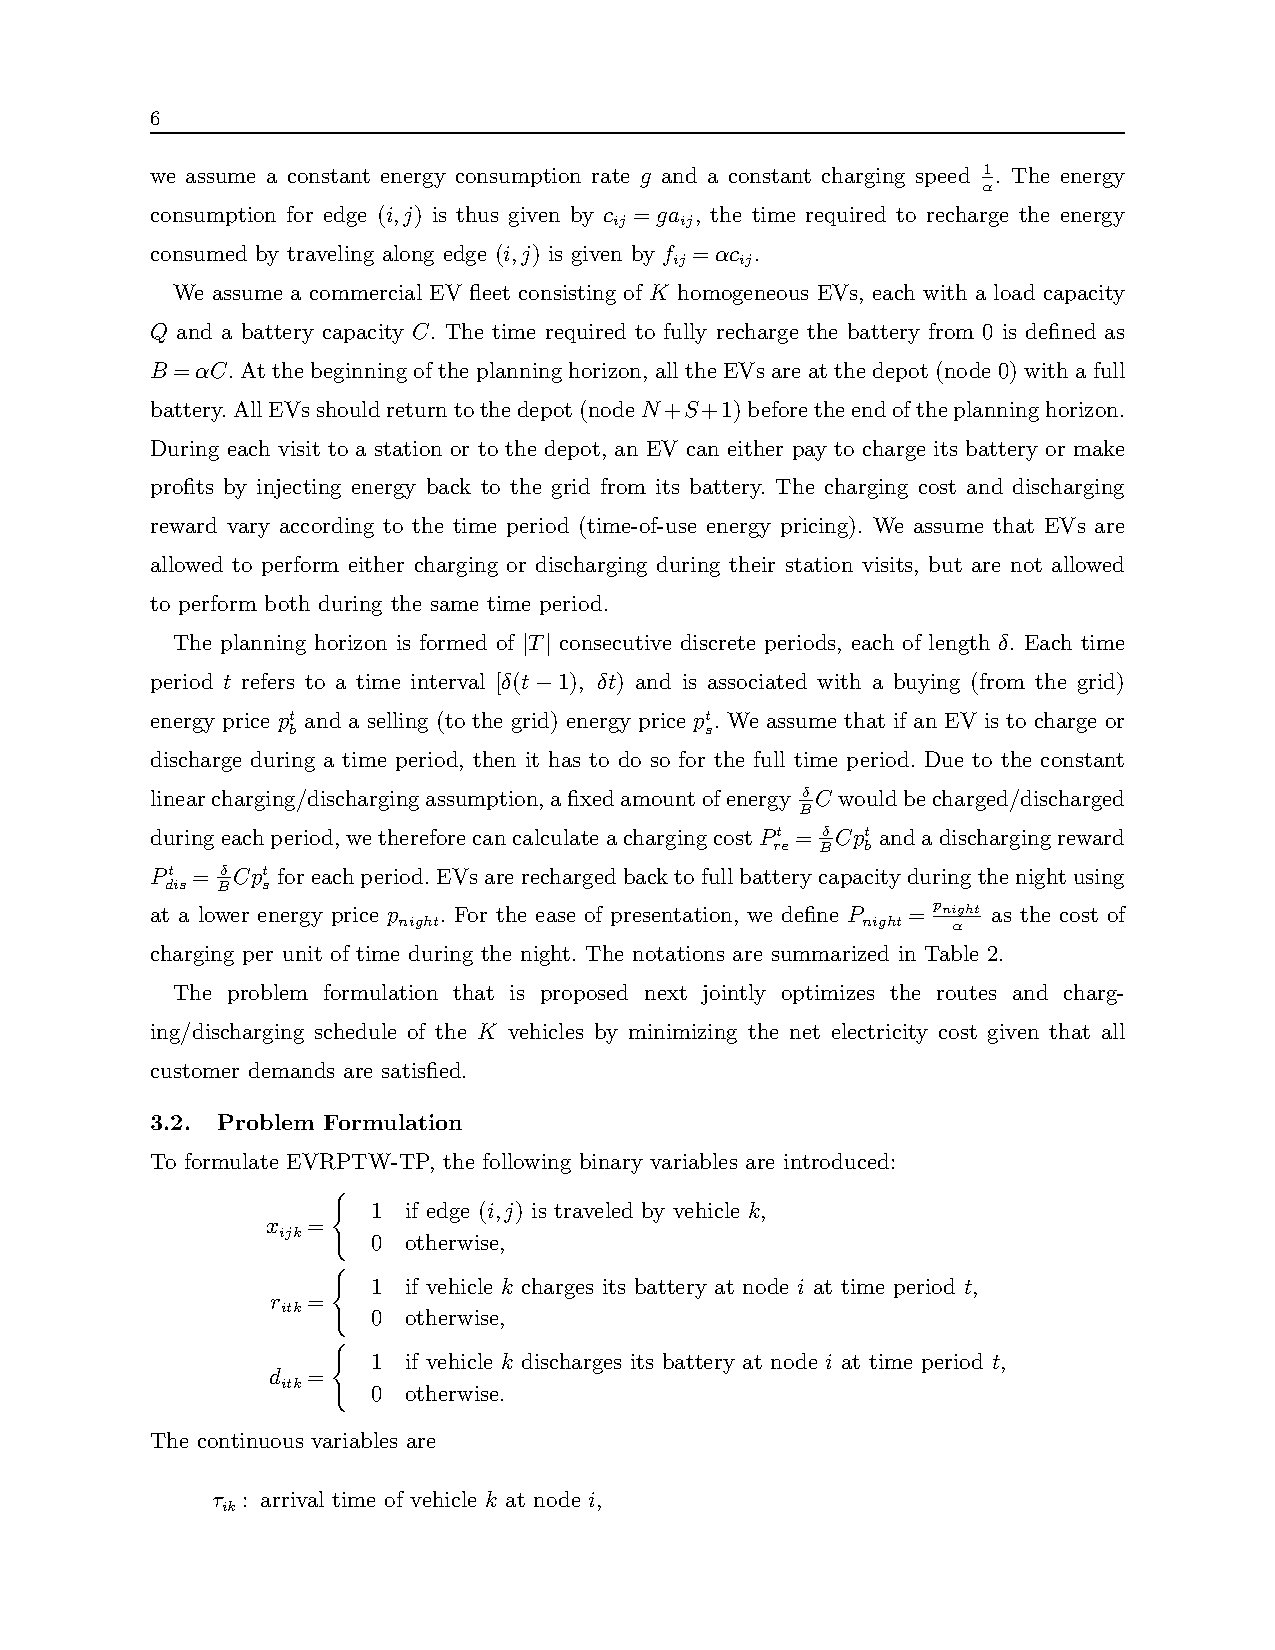
\includepdf[pages=-,scale=0.94,pagecommand={}]{source_excerpts/13_lin_2021_pages_6_9.pdf}

\end{document}
